\documentclass[conference,compsoc]{IEEEtran}
% *** CITATION PACKAGES ***
%
\ifCLASSOPTIONcompsoc
  % IEEE Computer Society needs nocompress option
  % requires cite.sty v4.0 or later (November 2003)
  \usepackage[nocompress]{cite}
\else
  % normal IEEE
  \usepackage{cite}
\fi


\usepackage{microtype}
\usepackage{booktabs} % for professional tables


\usepackage{graphicx} % "demo" option just for this example
\usepackage{subcaption}

\usepackage{booktabs,subcaption,amsfonts,dcolumn}
\newcolumntype{d}[1]{D..{#1}}
\newcommand\mc[1]{\multicolumn{1}{c}{#1}} % handy shortcut macro


\usepackage{booktabs,subcaption,amsfonts,dcolumn}
\newcolumntype{d}[1]{D..{#1}}


\usepackage[usenames, dvipsnames]{color}
\newcommand{\ts}{\textsuperscript}

\usepackage{graphicx}

\graphicspath{{/home/danai/Documents/ANN_2/images/Report1Exercise2/}{/home/danai/Documents/ANN_2/figures/}}
% *** GRAPHICS RELATED PACKAGES ***
%
\ifCLASSINFOpdf

\hyphenation{op-tical net-works semi-conduc-tor}

\usepackage{tabularx} % in the preamble
\begin{document}
%
\title{\line(1,0){250}\\Artificial Neural Networks and Deep Learning\\\line(1,0){250}}
%\title{[H02C4A] Artificial Neural Networks and Deep Learning}


\author{\IEEEauthorblockN{Danai Triantafyllidou}
\\
	\IEEEauthorblockA{Master of Artificial Intelligence, KU Leuven\\
	\\2018-2019
	\vspace{1cm}
	}
}

%\onecolumn
%\tableofcontents
%\listoffigures
% 
%\listoftables
\maketitle


\IEEEpeerreviewmaketitle
%\onecolumn


\thispagestyle{plain}
\pagestyle{plain}

\section{Supervised learning and generalization}

\subsection{Backpropagation in feedforward multi-layer networks}

\subsubsection{Experiments}
In this exercise, a feedforward neural network with one hidden layer is employed to approximate the function $y=sin(x^2)$. According to the universal approximation theorem, a single hidden layer is sufficient for any neural network to approximate any continuous function arbitrarily well. The theorem thus states that simple neural network architectures are universal approximators for the right number of parameters but it does not refer to the algorithmic learnability of these parameters.


The performance analysis includes the evaluation of the following training algorithms: gradient descent (\textit{traingd}), gradient descent with adaptive learning rate (\textit{traingda}), Fletcher-Reeves conjugate gradient (t\textit{raincgf}), Polak-Ribiere conjugate gradient (\textit{traincgp}), BFGS quasi Newton (\textit{trainbfg}), Levenberg-Marquardt (\textit{trainlm}) and Levenberg-Marquardt with Bayesian regularization (\textit{trainbr}). The effect of various parameters including the number of neurons in the hidden layer, the number of training epochs and the number of training examples is also examined. A second set of experiments, involved measuring the effect of adding random noise to the training data points. 

Optimization algorithms require that the weights of the network are initialized to random values. Additionally, in the case of batch learning randomness can be used by a learning algorithm while shuffling and selecting the training samples that will compromise each batch, resulting in different gradient estimates after each epoch. In order to evaluate and make meaningful comparisons among different combinations of training algorithms and parameters, it is useful to asses performance over a multiple-restart search. Therefore, for each training experiment the performance is measured by averaging both Regression-R values and training times over 10 runs and aggregated statistics are summarized in Figure~\ref{fig:res1}. Additionally, depending on how the weights are initialized, the algorithm may converge to a different local minimum. The weights of every training experiment were initialized every time to the same weight matrix, with a view to start the optimization always from the same point in the weight space. 
  
    \begin{figure*}[]
    
        \begin{subfigure}{0.33\linewidth}
            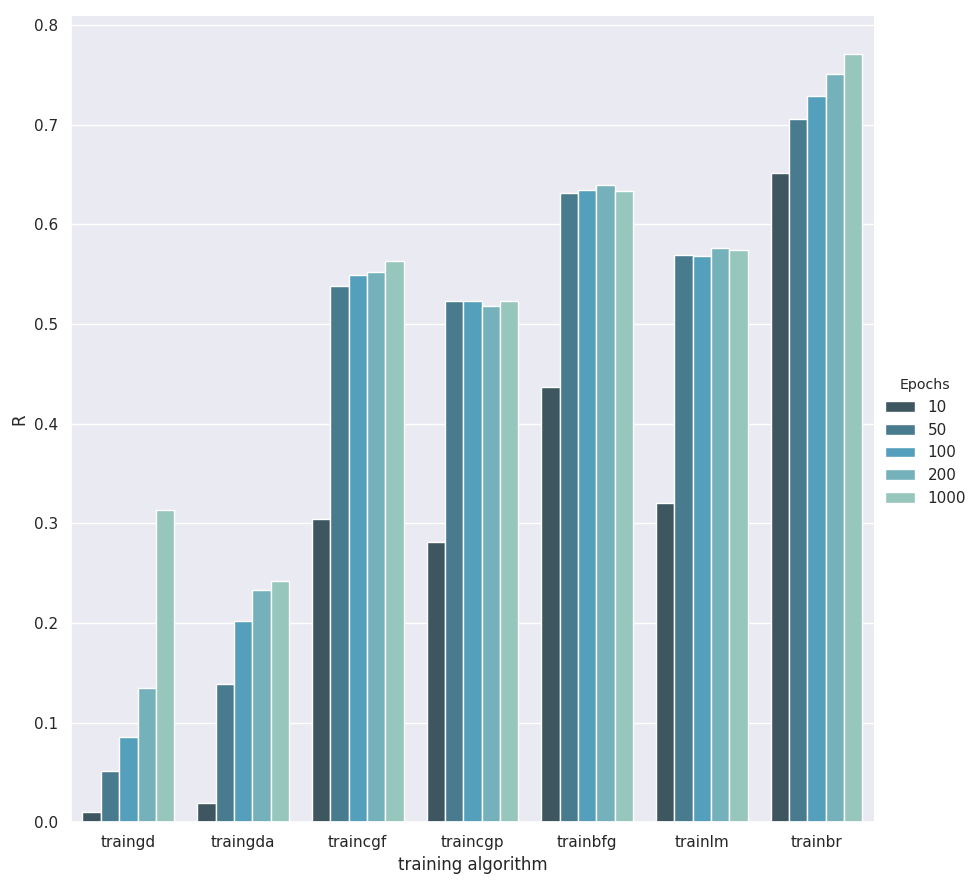
\includegraphics[width=\linewidth]{EpochsR}
            \caption{Number of epochs - R}
        \end{subfigure}
        \begin{subfigure}{0.33\linewidth}
            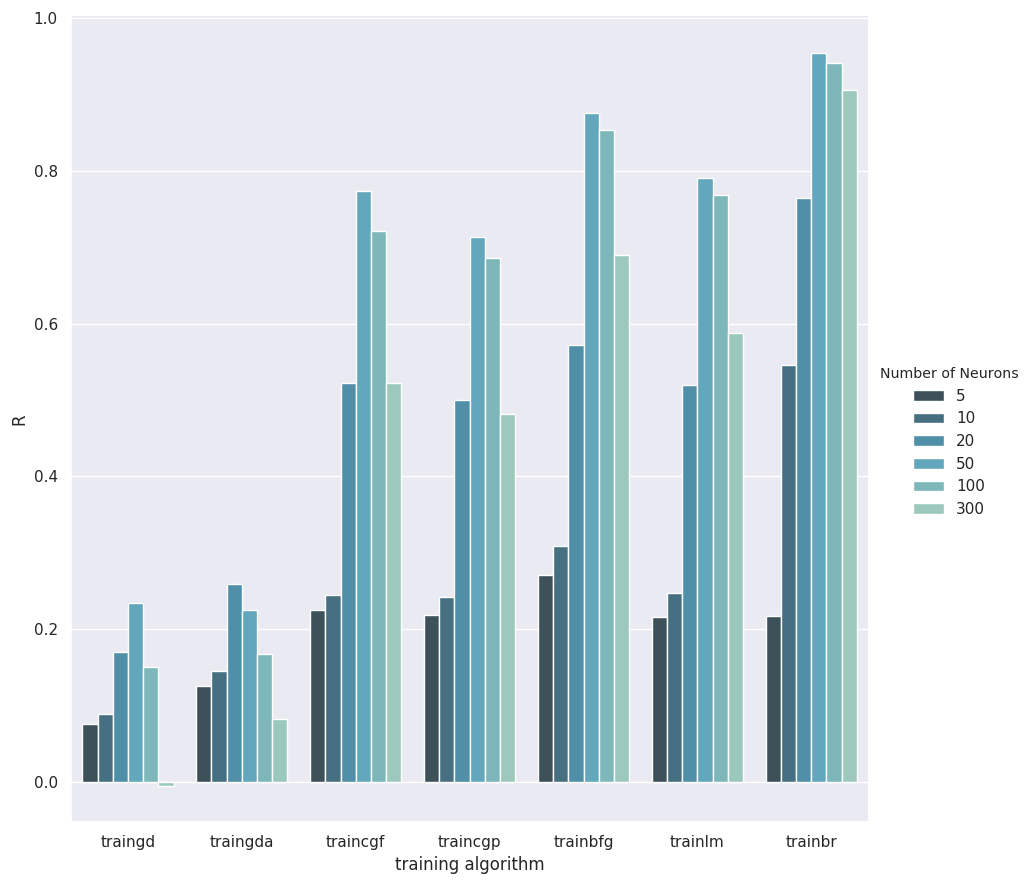
\includegraphics[width=\linewidth]{neuronsR}
            \caption{Number of hidden neurons - R}
        \end{subfigure}
        \begin{subfigure}{0.33\linewidth}
            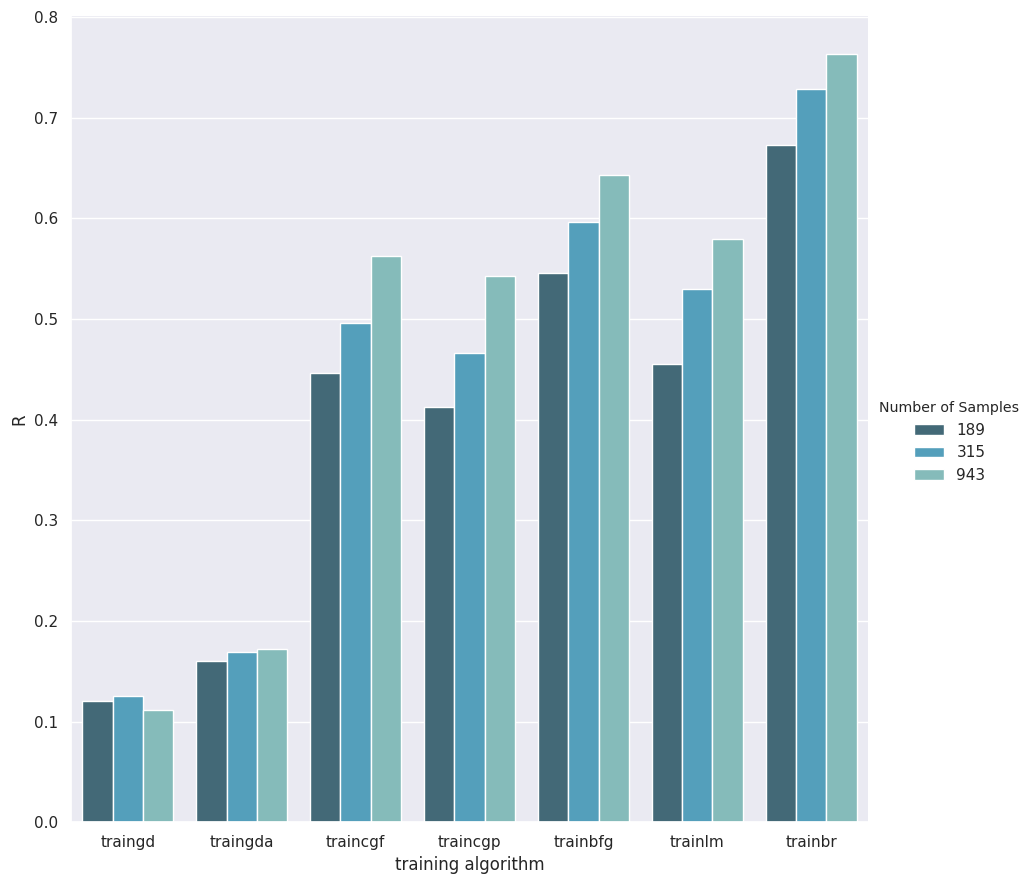
\includegraphics[width=\linewidth]{SamplesR}
            \caption{Number of samples - R}
        \end{subfigure}


		\begin{subfigure}{0.33\linewidth}
            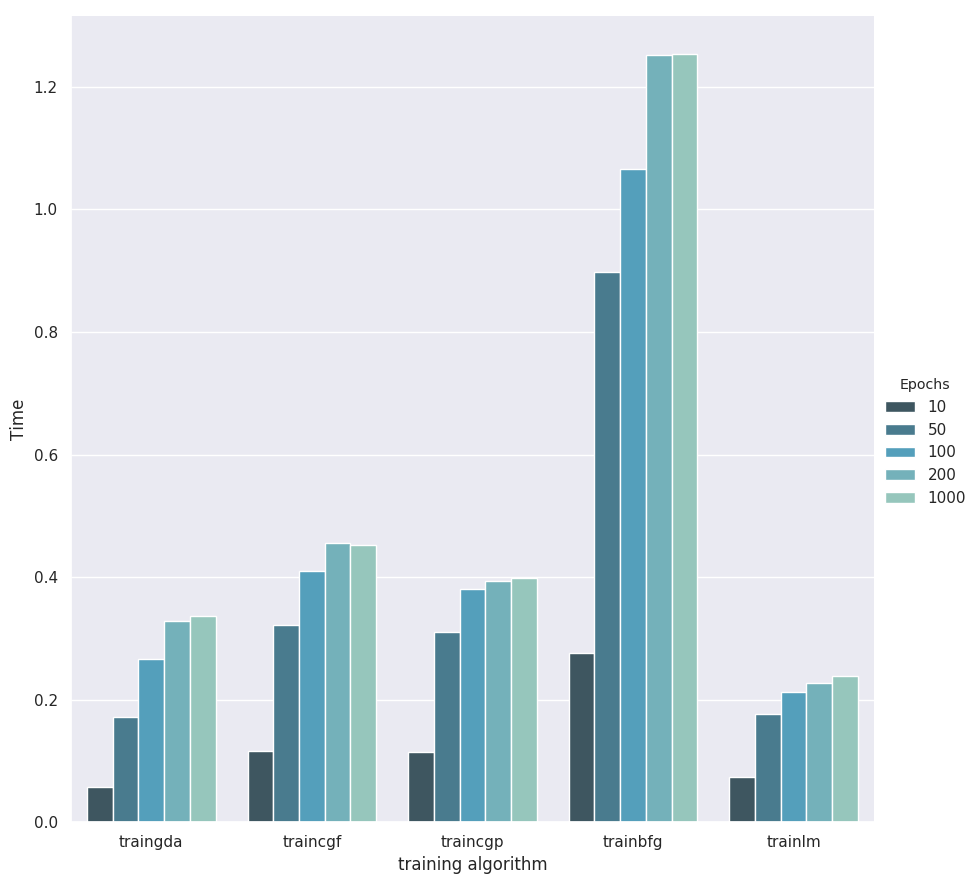
\includegraphics[width=\linewidth]{EpochsTime}
            \caption{Number of epochs - Time}
        \end{subfigure}
        \begin{subfigure}{0.33\linewidth}
            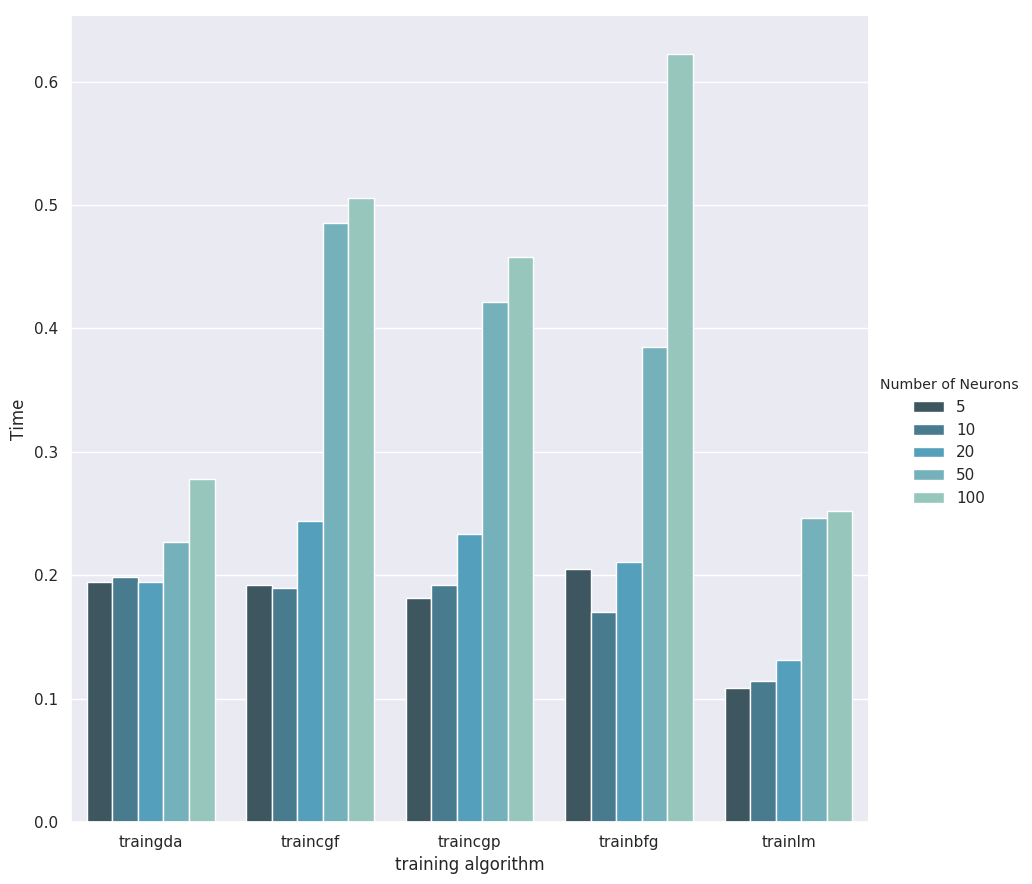
\includegraphics[width=\linewidth]{neuronsTime}
            \caption{Number of hidden neurons - Time}
        \end{subfigure}
        \begin{subfigure}{0.33\linewidth}
            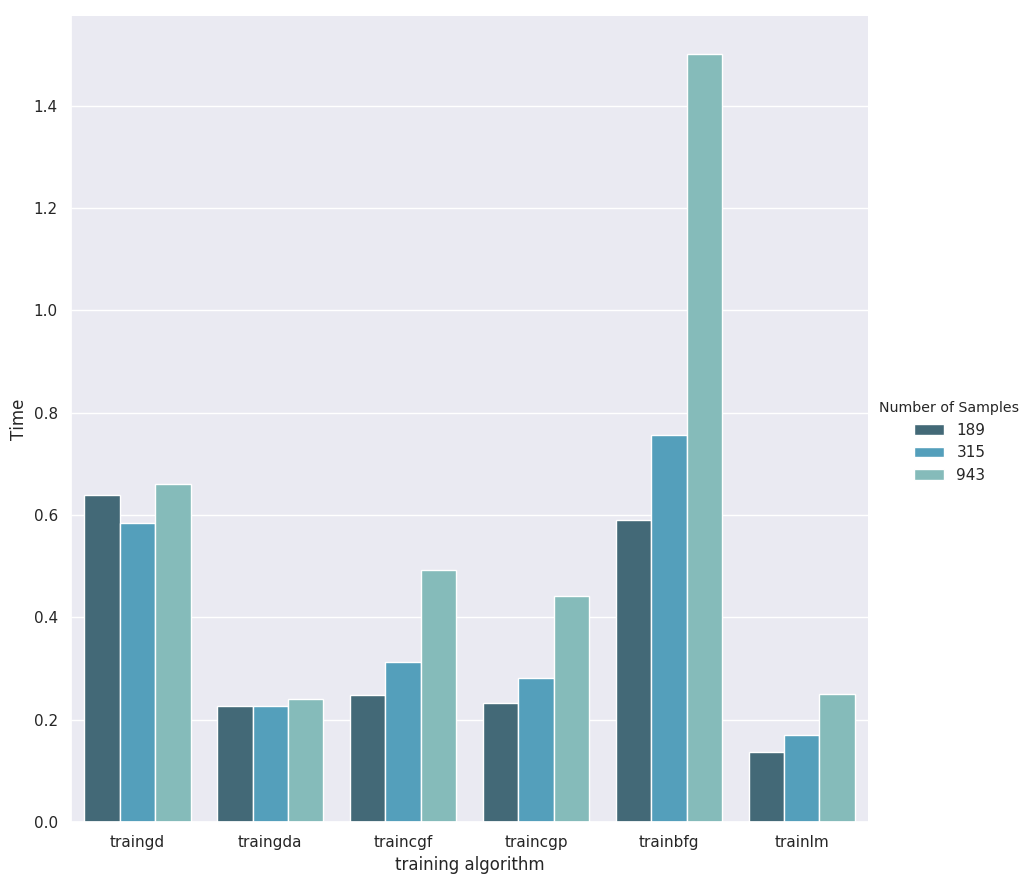
\includegraphics[width=\linewidth]{SamplesTime}
            \caption{Number of samples - Time}
        \end{subfigure}
   	
        \caption{ Varying the effect of various parameters and measuring performance in terms of R value and training time.}       
   
        
        \label{fig:res1}
    \end{figure*}
\textbf{Number of neurons:} The number of hidden neurons of the neural network was varied from 5 to 10, 20, 50, 100 and 300. The first thing to note is that adding more neurons, increases training time as the model becomes more complex and requires the training of more parameters (Figure ~\ref{fig:res1}-e). Using an insufficient number of hidden neurons will impact the generalization ability of the model as the model becomes less expressive and fails to capture the underlying relationship between the input and the output. According to the traditional bias-variance trade-off, the last situation is a high bias setting where the model is likely to underfit the available data. On the other hand, using an extremely large number of hidden units will increase the variance of the model and could possibly lead to overfitting as the neural network will over-estimate the complexity of the target problem and will fail to generalize well to new data. Indeed, for most training algorithms, increasing the number of hidden neurons to more than 50 produces a worse result in terms of R values (Figure~\ref{fig:res1}-b). Finally, according to the Occam's principle the ideal number of parameters should be determined by choosing the simplest model that performs best, in this case a neural network with 50 hidden units. 

\textbf{Number of epochs:} During one epoch, the complete set of training vectors are presented to the neural network and the weights are adjusted accordingly. The number of epochs was varied from 10 to 50, 100, 200 and 1000. As expected, if the network is trained for very small number of epochs (e.g. 10) the optimization does not have enough time to converge to an optimum solution (Figure~\ref{fig:res1}-a). As the number of epochs increases, the algorithms are able to further explore the search space and find the minimum of the objective function. After the algorithm has converged to a local or global minimum, increasing the number of epochs should not be encouraged since it may give rise to overfitting.

\textbf{Number of samples:} Increasing the number of samples (from 189 to 315 and 943) evidently improves the performance of the training algorithms since the neural network is provided with more information about the task it is required to solve. However, it should be noted that once the algorithm reaches a global optimum, additional samples are an overhead since they severely increase the training time, especially for BFGS quasi Newton where training time is increased from 0.59 sec for 189 samples to 0.78 and 1.5 for 315 and 943 samples respectively.

\textbf{Noisy data:} The level of Gaussian noise added to the training data is expressed as the standard deviation $\sigma$ and was varied from 0 to 0.4. As illustrated in Figure~\ref{fig:noise1}, increasing the level of noise, lowers the R value of the predicted and the groundtruth values. It is also observed that the Levenberg-Marquardt with Bayesian regularization algorithm performs better than all the evaluated algorithms for all the different noise levels.

 %From Figure~\ref{fig:noise}, it is evident that the Levenberg-Marquardt with Bayesian regularization algorithm is more robust to noise than all the algorithms included in the evaluation.
\subsubsection{Conclusions}
From Figures~\ref{fig:res1} (a-c), it is clear that gradient descent and gradient descent with adaptive learning rate perform significantly worse compared to all other training algorithms. This can be explained by the fact that these algorithms do not exploit any information concerning the second order derivatives of the objective function. Furthermore, the performance of the gradient descent algorithm depends heavily on the choice of the learning rate parameter. A very high learning rate allows for greater adaptations in the weight matrix of the neural network and is more likely to fail to converge to a minimum or may even diverge. On the other hand, a small learning rate will lead to very slow optimization since it imposes small changes to the model's weights.

 In Table~\ref{fig:res1t}, the average training time, R-value and mean squared training error (MSE) are reported over 10 different runs for the noise free set of experiments. Clearly, gradient descent and gradient descent has a deteriorated performance with an average training time of 0.78, R-value of 0.12 and MSE of 16.10. Gradient descent with adaptive learning rate slightly improves training speed and the correlation coefficient but not to a significant level. 

While gradient descent only takes into account the gradient of the cost function, conjugate gradient algorithms also exploit information about the search direction of the previous iteration. When the gradient keeps pointing in the same direction, this will increase the size of the steps taken towards the minimum. The performance of the Polak-Ribiere conjugate gradient and the Fletcher-Reeves conjugate gradient algorithms is very similar both in terms of speed and R-values. As illustrated in Figure~\ref{fig:noise1}, the Fletcher-Reeves algorithm slightly outperforms the Polak-Ribiere algorithm.

An advantage of quasi-Newton methods is that they take into account information regarding the second order derivative
s which  gives a better idea of the geometry of the landscape that is being optimized. An approximation of the Hessian matrix is computed using updates specified by gradient evaluations. Indeed, BFGS quasi Newton gives satisfying results and seems to be more robust to noise than both steepest descent and conjugate gradient algorithms (Figure~\ref{fig:noise1}). The only downside of the latter algorithm is that training time increases severely as more samples are included in the training set. As illustrated in Table~\ref{fig:res1t}, the BFGS quasi Newton suffers from a deteriorated speed performance but achieves a better average R-value.

A common problem that optimization algorithms are facing is that of an ill-conditioning Hessian matrix, which arises as the number of parameters grows. An ill-conditioning Hessian matrix poses a problem to the optimization process since the computation of the inverse of the Hessian might introduce significant numerical instability. Levenberg-Marquardt is a training algorithm that addresses this problem by adding the expression $\lambda I$ to the Hessian matrix. As a result, the Hessian matrix becomes a full rank matrix and can be inverted even in the case of ill-conditioning. One of the main drawbacks of this algorithm is that the Hessian matrix still needs to be stored and may lead to excessive memory consumption. The main advantage of this algorithm, as shown in Table~\ref{fig:res1t}, is that it is very fast, outperforming all other optimization methods in terms of speed with an average training time of 0.22 seconds.

In a Bayesian setting, instead of a single weight point in the weight space, we characterize learning by a probability distribution of  network weights. As a consequence, it is possible to characterize the uncertainty of each prediction. The Levenberg-Marquardt with Bayesian regularization algorithm extends the cost function as $M(w) = \beta E_D(w)+\alpha E_W(w)$, where the second term is related to the prior distribution of the weights.  The two parameters $\alpha$ and $\beta$ indicate whether the learning process should emphasize towards minimizing the error or minimizing the values of the weight matrix. In Figure~\ref{fig:res1}, it is clearly illustrated that this algorithm outperforms all the training algorithms in terms of the average R-values and is more robust to noisy input. Finally, Table~\ref{fig:res1t} shows that the average R-value for the noisy free set of experiments is 0.76, surpassing the Levenberg-Marquardt algorithm with a margin of 0.19.

All experiments for this exercise were conducted using MATLab (version r2018b) on a NVIDIA GTX 1050 GPU. For the Levenberg-Marquardt with Bayesian regularization algorithm (trainbr) the reported average training time in Table~\ref{fig:res1t} refers to computations executed in CPU since there is no MATLAB implementation for GPU support.

\begin{figure}
\centering
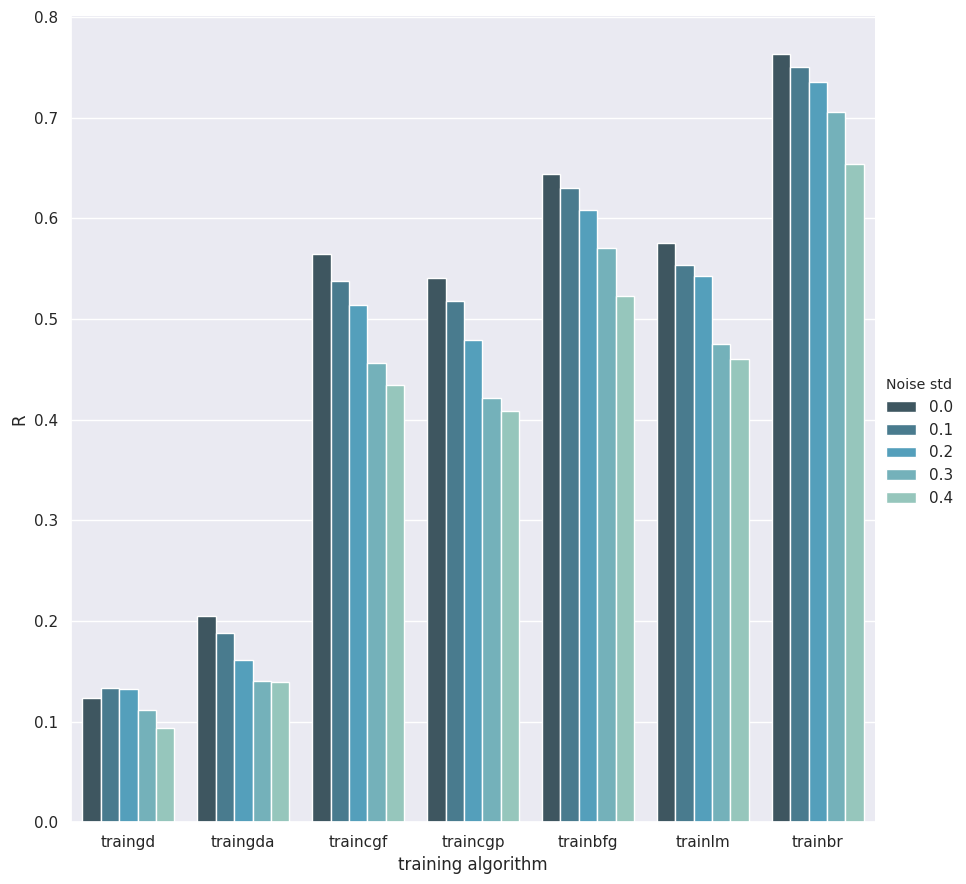
\includegraphics[width=7cm]{NoisestdR.png}
        \caption{Investigating the effect of adding random noise to training data with standard deviation values from 0.1 to 0.4.}
\label{fig:noise1}
\end{figure}
 


   
\begin{table}
\centering
%\begin{tabular}[t]{@{} l c *{3}{d{1.7}}d{3} @{}}
\begin{tabularx}{6cm}[t]{l l l l l l l l l}
\toprule

 &Time &   R-value &MSE \\
\midrule
  traingd &0.78  & 0.12& 16.10  \\
                                          
 traingda & 0.24 &0.20  &1.30 & \\
                                               
 traincgf & 0.39 &   0.56 & 0.35 \\
 traincgp & 0.35 &   0.54 & 0.41 \\
 trainbfg &1.31 &   0.64 & \textbf{0.26} \\
  trainlm &\textbf{0.22}&   0.57 & 0.32 \\
  trainbr &4.11\footnote{\label{note1}CPU time}&  \textbf{0.76} & 1.54 \\

\bottomrule
\end{tabularx}

\caption{Mean performance over 10 runs for different optimization algorithms.
 \\
 }
\label{fig:res1t}
\end{table}


\subsection{Function approximation using feedforward multi-layered networks}

\subsubsection{Dataset}
In this exercise, the objective is to approximate a nonlinear function $f(X1,X2)$ using a multi-layered neural network. The function we are trying to approximate is a combination of 5 nonlinear functions  $f_1, f_2,...,f_5$ where $f(X1,X2) = 7 f_1(X1, X2)+ 5 f_2(X1, X2) + 5 f_3(X1, X2) +3 f_4(X1, X2)+ 3 f_5(X1, X2)$.

The initial dataset consists of 13.600 three dimensional data points but the exercise requires that the training, validation and test sets will consist of 1000 data points each. In order to properly estimate the generalization error, tests must be carried out on a sample of the data that is statistically independent from that used during training. Furthermore, sampling from a small neighborhood will result in biased estimates of the generalization error since the model will likely fail to capture the characteristics of the data observed in a broader domain. Shuffling the data is the simplest way to avoid this and ensure that all three partitions follow the same distribution.
The training, validation and test surfaces are visualized in Figure~\ref{fig:sur}.


        \begin{figure*}[]
        \begin{subfigure}{0.33\linewidth}
            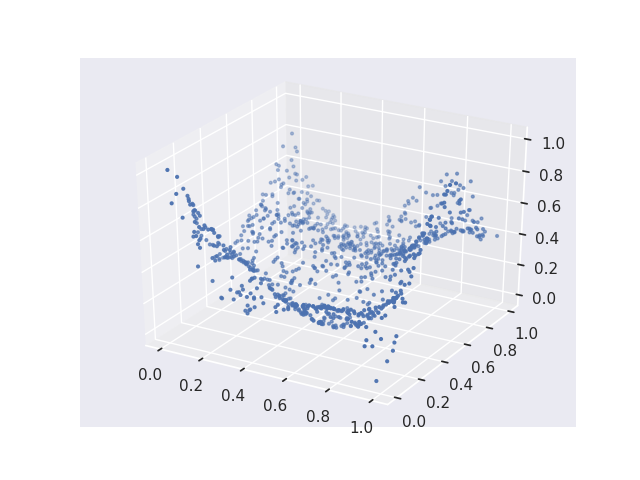
\includegraphics[width=\linewidth]{trains}
            \caption{training}
        \end{subfigure}
        \begin{subfigure}{0.33\linewidth}
            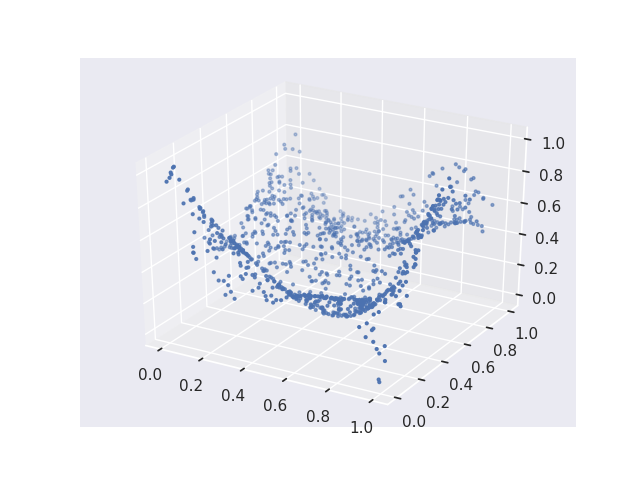
\includegraphics[width=\linewidth]{vals}
            \caption{validation}
        \end{subfigure}
        \begin{subfigure}{0.33\linewidth}
            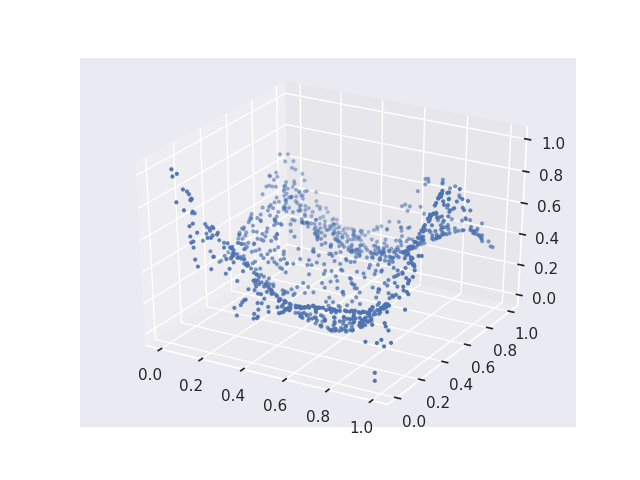
\includegraphics[width=\linewidth]{tests}
            \caption{test}
        \end{subfigure}
        \caption{Visualizing the personal regression surface}
        \label{fig:sur}
\end{figure*}

\begin{table*}\centering
%\ra{1.3}
\begin{tabular}{@{}rrrrrrrccrrrcrrr@{}}\toprule
& \multicolumn{4}{c}{Train} & \phantom{abc}& \multicolumn{2}{c}{Validation} &
\phantom{abc} \\
\cmidrule{2-5} \cmidrule{7-9} \cmidrule{10-12}
&  & tansig & logsig    &&  & tansig &   logsig \\ \midrule
traincgf && 0.0017 & 0.0024 && &0.0064& 0.0070\\
\\
traincgp && 0.0022&0.0039&&&0.0067&0.0085\\
\\


trainbfg&&\textbf{0.0012}&0.0013&&&\textbf{ 0.0017}&0.0056\\
\\
trainlm&&0.0018&0.0015&&& 0.0060&0.0059\\
 
\bottomrule
\end{tabular}
\caption{MSE for the MLP with 100 neurons measured over 10 runs in the training and validation sets for the personal regression task}
       \label{tbl:reg1}
\end{table*}


   
\begin{table*}
\centering
\begin{subtable}[t]{0.4\textwidth}
%\begin{tabular}[t]{@{} l c *{3}{d{1.7}}d{3} @{}}

\begin{tabular}[t]{l l l l l l l l l}
\toprule

\# units & params &$MAE$ &   $MSE$  &$R^2$\\
\midrule

                        
 100 & 401 &0.064 & 0.0049& 0.80 \\

\bottomrule
\end{tabular}
\end{subtable}
\caption{Performance of regression measured in the test set for the MP with 100 neurons
 }
\label{fig:reg}
\end{table*}

   \begin{figure*}[]
        \centering
        \begin{subfigure}{0.4\linewidth}
            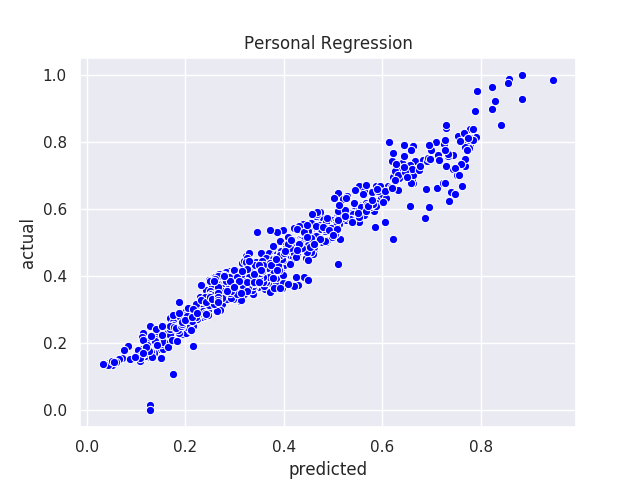
\includegraphics[width=\linewidth]{regression}

        \end{subfigure}
    
        
        \caption{Predicted against actual values for the personal regression task}
        \label{fig:regsum}
\end{figure*}

      \begin{figure*}[]
        \centering
        \begin{subfigure}{0.33\linewidth}
            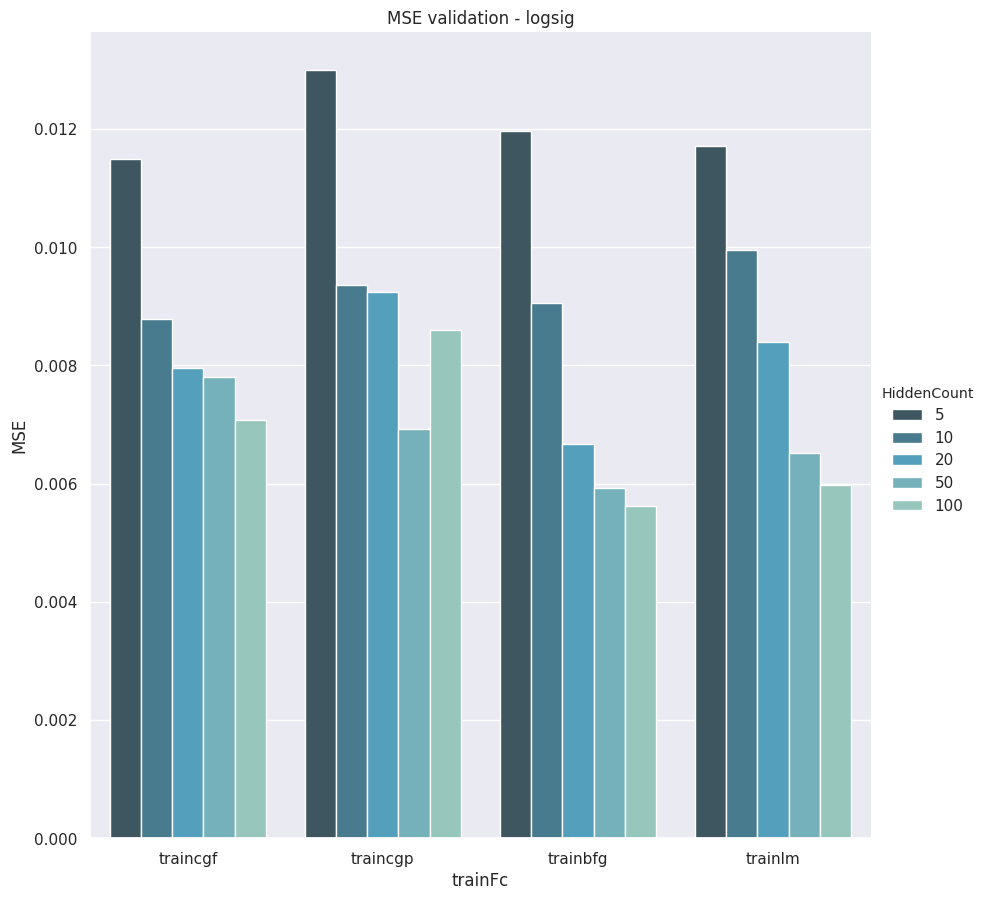
\includegraphics[width=\linewidth]{valmse_logsig}
            \caption{logsig}
        \end{subfigure}
        \begin{subfigure}{0.33\linewidth}
            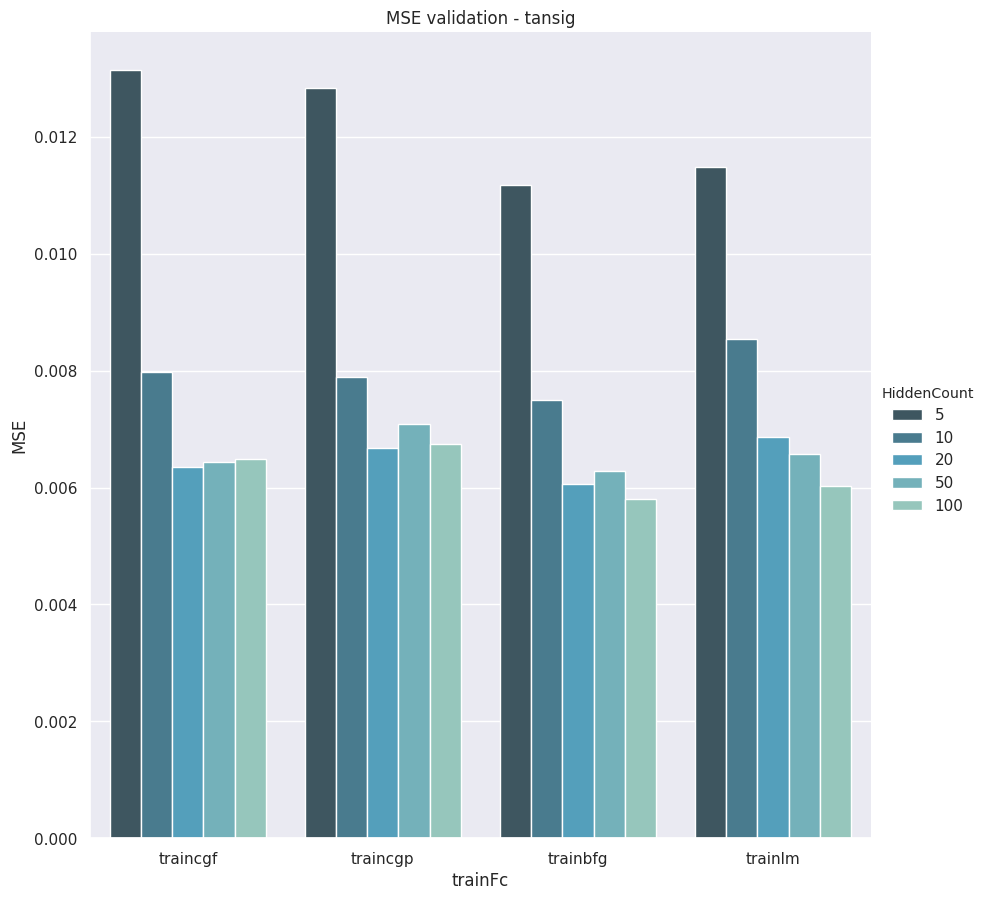
\includegraphics[width=\linewidth]{valmse_tansig}
            \caption{tansig}
        \end{subfigure}
        
        \caption{Validation performance for the personal regression task}
        \label{fig:regsum}
\end{figure*}



The validation set should be used to assess the performance of the network during training and tune the hyperparameters of the model. Since the validation set includes data independent of that used for training, validation  performance reflects the generalization ability of the model.  The validation should not be confused with the test set which is meant to assess the performance of a fully-specified model.  If the use of a test independent set is omitted, the obtained error estimates will become over-optimistic over multiple training attempts since the model is also tuned on scoring well on the validation set.



\subsubsection{Training \& Performance Assessment}
 
%The first set of experiments involved training a multi-layered perceptron with one hidden layer 
% 
%Even though it is theoretically possible to approximate any continuous function by deploying a neural network with one hidden layer, determining the right number of neurons in the hidden layer may be a challenging issue. Additionally, the universal approximation theorem states that a single hidden layer is sufficient but only if the input is continuous and within a compact space. Therefore, since the underlying properties of the function we are trying to approximate are unknown, it would be a good idea to use an architecture with multiple layers that allows to learn more detailed and abstract representations. Every layer in the architecture adds a new level of non-linearity and allows to represent more complex features, possibly composed of low level features. 

The bias-variance trade-off in machine learning suggests that as the number of trainable parameters grows the variance of the model is increased (thus also increasing the risk of overfitting) while the bias is decreased. This leads to the conclusion that the simplest model that performs best should be chosen. The first set of experiments involved training a neural network architecture with one hidden layer. Since it is theoretically possible to approximate any continuous function with one hidden layer, this choice seems plausible for a simple regression task with a two dimensional input. A statistical evaluation similar to the one in the previous section is used. In particular, the performance is measured in the validation set by averaging the mean squared error (MSE) over 10 runs. The number of neurons in the hidden layer was varied from 5, 10, 20, 50, and finally 100. Two different activation functions were tested: the hyperbolic tangent sigmoid function (\textit{tansig}) and the log-sigmoid function (\textit{logsig}). Figure~\ref{fig:regsum} summarizes the validation performance. It is observed that the architecture with 100 neurons achieves the lowest MSE score in almost all cases. In Table~\ref{tbl:reg1}, the MSE in the training and validation set is reported for the architecture with 100 neurons measured over 10 runs. The best performance in the validation set is achieved using the tangent activation function and the BFGS quasi Newton optimization algorithm. 





After selecting the number of hidden neurons, the optimization algorithm and the activation function of the network, the performance is assessed in the test set. The model achieves a mean squared error (MSE) of 0.049, a mean absolute error (MAE) of 0.028 and a R-squared value of 0.80. As expected, the training error is the lowest and the validation error is slightly higher than the training error. A second set of experiments was also conducted that involved training an architecture with three hidden layers. The number of neurons in each of the hidden layers was varied from 50, to 100 and finally 200. This set of experiments was mainly focused on examining the performance of different optimization algorithms available in the Keras library, namely Adam, Adadelta, Adagrad, Nadam and Adamax. The best validation MSE score of 0.0008 was achieved using Adam and 200 neurons in each one of the three hidden layers. The training and validation plots as well as the MSE, MAE and $R^2$ scores have been included in the Appendix.




  
    
%\texttt{ while varying the number of the neurons in each hidden layer from 50 to 100 and finally to 200 neurons. During all the experiments the network was trained using Adam optimization algorithm for 40 epochs. Figure~\ref{fig:reg2} illustrates the Mean squared loss for the training and validation sets for the three different model architectures. A second set of experiments focused on comparing different optimization algorithms available in the Keras library, namely Adagrad, Adadelta and Adam, Adamax and Nadam. 
%
%\textbf{Number of neurons} A statistical evaluation similar to the one in the previous section is used. In particular, the performance is measured by reporting the mean values of 4 different metrics over 10 runs. Table~\ref{fig:reg} summarizes the mean value for the Mean absolute error (MAE), Mean Squared Error (MSE) and $R^2$ score. The architecture with the 200 neuron in each one of the three hidden layers performs best since the MAE and MSE scores are lower and the $R^2$ coefficient raises to 0.967}


%adagrad:
%MAE 0.04881102815844612
%MSE 0.004339284660518322
%RMSE 0.06544940814095829
%R 0.8410336738853649

%adadelta:
%MAE 0.07519869954553288
%MSE 0.01008285994888901
%RMSE 0.10040603993931302
%R 0.6306222503937258

%adam





\section{Recurrent neural networks}


\subsection{Hopfield Network}


A hopfield neural network is an abstract model of image retrieval designed to store patterns $\xi \in R^N$, with $\xi=[\xi_1, \xi_2,...,\xi_N]^T$ where $\xi \in \{-1,+1\}$. It is a type of recurrent neural network where the dimensionality of the input and the output should match and the output from time $t$ is used as an input to step $t+1$. The Hopfield network consists of a set of N interconnected neurons which update their activation values either asynchronously and independently of other neurons or synchronously. Every neuron $i$ can have two states a firing state if $S_i=1$ and a non-firing state if $S_i=-1$.
The dynamics of the system evolve in discrete time $t$ and the update for each neuron can be described as:

\begin{equation}
S_i(t+1) = sign(\sum_{j=1}^{N} w_{ij}S_j(t)), i = 1,...N
\end{equation}
where $w_{ij}$ refers to the weight connection between neuron $i$ and $j$ and $S_j(t)$ is the state of neuron $j$ at time $t$. 

For a suitable choice of the weight matrix $W$ patterns can be retrieved by the dynamics defined in equation 1, applied to all $N$ neurons of the system. According to the Hebb rule, in order to store $\mu$ patterns the weights of each connection should be chosen as $w_{ij} = \frac{1}{N} \sum_{\mu=1}{p}\xi_i^\mu\xi_j^\mu$. The Hopfield network correctly represents a pattern $\mu$ if the state of each neuron $S_i$ is equal to the $i^{th}$ component of pattern $\xi_i^{\mu}$. In other words $sign(W\xi)=\xi$. In the ideal case, equation 1 should converge to a fixed point $\mu$ which is most similar to the initialization state $S(t_0)$. These points are called equilibrium points.

Hopfield networks can work as an associative memory in a sense that they are able to retrieve the values associated with the stored patterns even in the presence of noise. 
The dynamics of equation 1 is "attracted" to fixed points similar to one of the memorized patterns. These points are called attractors and are located at the local minima of the energy function:

\begin{equation}
H = -\frac{1}{2}\sum_{ij}w_{ij} S_iS_j
\end{equation}

A well known problem of Hopfield networks is that they may store additional unwanted patterns that are called spurious attractor states. These states are also local minima of the energy function but are not explicitly provided during the learning process. An exampe of an spurious attractor is the storage of pattern $-\xi^\nu$ whenever pattern $\xi^\nu$ is stored. Figure~\ref{fig:hop2} shows some examples of spurious attractor states. Finally, in figure~\ref{fig:hop} a two dimensional Hopfield network with attractors $(1,1), (-1,-1)$ and $(1,-1)$ is created. 



 \begin{figure}
	\begin{subfigure}{8cm}
            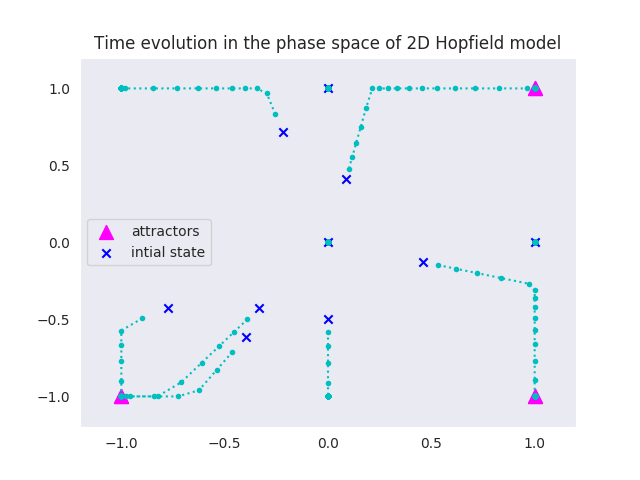
\includegraphics[width=\linewidth]{hop}          
        \end{subfigure}
        \caption{Time evolution in a 2D Hopfield network}               
        \label{fig:hop}
    \end{figure}
\begin{figure}   
\centering
\minipage{0.07\textwidth}
  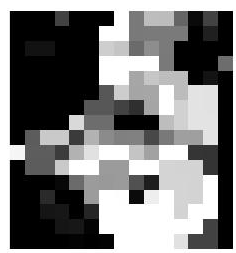
\includegraphics[width=\linewidth]{att/1}
\endminipage
\vspace{1mm}
\minipage{0.07\textwidth}
  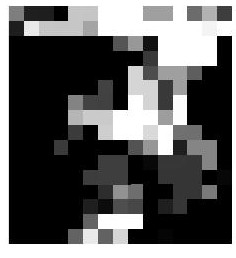
\includegraphics[width=\linewidth]{att/2}
\endminipage
\vspace{1mm}
\minipage{0.07\textwidth}%
  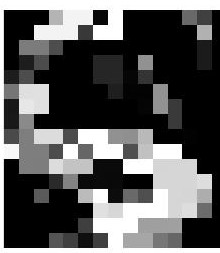
\includegraphics[width=\linewidth]{att/3}
\endminipage
\minipage{0.07\textwidth}%
  \includegraphics[width=\linewidth]{att/4}
\endminipage
\minipage{0.07\textwidth}%
  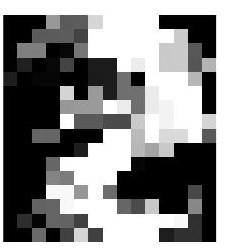
\includegraphics[width=\linewidth]{att/5}
\endminipage

\caption{Exampes of spurious attractor states in the Hopfield network}
\label{fig:hop2}
\end{figure}
In this exercise, a Hopfield neural network is deployed to retrieve digit patterns from 0 to 9. Digit patterns are encoded as images of size $16 \times 15$ but are reshaped as 240 dimensional vectors. Since the dimension of the input should match the dimension of the output the network should consist of 240 neurons. The network is expected to retrieve the memorized pattern and output an attractor state which in this case should be the equivalent digit image that has been stored in the memory. In order to examine the effect of adding more noise to the input states, 10 images were randomly selected so that each one corresponds to one different digit from 0-9. The number of iterations was varied from 5 to 15, 30 and finally 60. The noise level was also increased from 1 to 5, 10, 15 and 20 and results measured over 100 runs are presented in Figure~\ref{fig:hop2}.

 There are three different situations that may occur: the network converges to the correct digit state, the network converges to a wrong digit or the network fails to converge to a pattern associated with a digit. A larger number of iterations ensures that the network will converge to a state possibly associated with a digit but there is no guarantee that this digit will always be the correct one. This situation is visualized in Figure~\ref{fig:hop2} (c) where it is shown that the number of failed retrievals decreases as the network is simulated for more iterations. In cases where there is no noise, the network can always retrieve the correct digits. As the noise level is increased the retrievals become less accurate as the number of incorrect retrievals gets higher while the number of correct retrievals decreases. This tendency is described in Figures~\ref{fig:hop2} (a) and (b).
 
        \begin{figure*}[]
        \centering
        \begin{subfigure}{0.30\linewidth}
            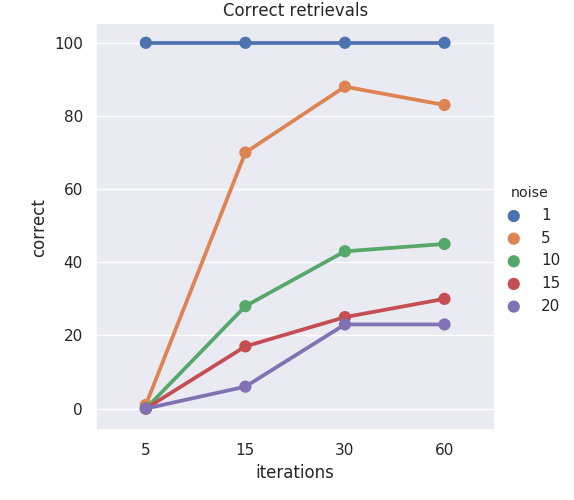
\includegraphics[width=\linewidth]{hop/correct_retrivals100}
            \caption{correct}
        \end{subfigure}
         \begin{subfigure}{0.30\linewidth}
            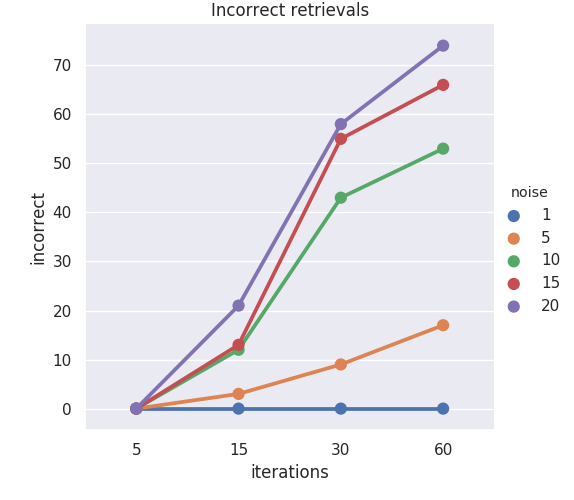
\includegraphics[width=\linewidth]{hop/incorrect_retrivals100}
            \caption{incorrect}
        \end{subfigure}  
        \begin{subfigure}{0.30\linewidth}
            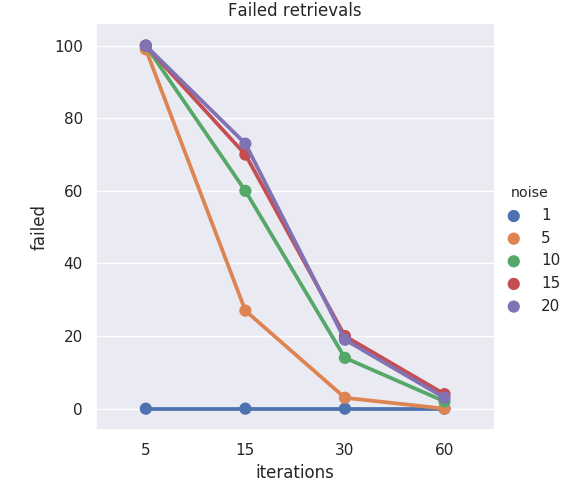
\includegraphics[width=\linewidth]{hop/Failed_retrivals100}
            \caption{failed}
        \end{subfigure}
		        
        \caption{Number of correct (a), incorrect (b) and failed (c) digit retrievals for the hopefield network}
        \label{fig:hop2}
\end{figure*}






\subsection{Time series prediction using Recurrent Neural networks}


\subsection{Time series prediction}

The objective of this exercise is to train a) a Recurrent multi-layered perceptron (MLP) with one hidden layer and b) a Long Short-Term memory network (LSTM) to perform time series prediction. The data is set A from Santa Fe Time Series prediction competition \cite{santafe}. The training set consists of 1.000 points recorded from a frar-Infered (FIR) laser in a chaotic state, with the assignment being to predict the next 100 points. 
Unlike regression modeling, time series prediction adds the complexity of a sequence dependence among the input variables. The task can be described as using the currently available points $y_k,y_{k-1},...,y_{k-p}$ to predict the future point $\hat{y}_{k+1}$.

In the case of the MLP, the network is trained in a feedforward fashion using back propagation. Since the structure of this model allows to predict only one step ahead in time, the network is converted to a recurrent model and the estimated values $\hat{y}_k$ are used iteratively to shift the input and predict the future points. A typical LSTM architecture involves the training of three different weight matrices $W_i$, $W_f$ and $W_o$ each one multiplied with the activations of three different units: a forget gate $f$, an input gate $i$ and an output gate $o$. Each one of these gates regulate the information flowing to a memory unit called cell. The forget gate can be described by the equation $f_t=\sigma(W_fx_t+U_fh_{t-1}+b_f)$ where $h_{t-1}$ is the previous state, $x_t$ is the current input. The last equation simply filters the input information and it outputs a number between 0 and 1 that indicates whether the current state should be memorized. Similarly to the forget state, the input and output gates model the significance of the information entering and exiting the cell and can be described as $i_t = \sigma(W_ix_t+U_ih_{t-1}+b_i)$ and $o_t=\sigma(W_{o}x_{t}+U_{o}h_{t-1}b_o)$. Finally, the hidden state $h_t$ that describes the information forwarded to the next state $t+1$ is computed as $h_t=o_t\circ tanh(c_t)$.
 
 
\subsubsection{Experimental Setup} 
The problem of time series prediction requires to make two critical design choices, first the number of neurons in the hidden layer and secondly the choice for the parameter $p$ that determines the number of points used to forecast the future prediction. Using a different delay step $p$ requires to split the 1.000 points to $p$ dimensional vectors. Thus, the choice of $p$ also affects both the feature dimension and the number of training examples provided to the network. For example, for $p=20$ the 1000 training points would be split into 980 examples of dimension 20, while for $p=100$ we obtain 900 examples of dimension 100. 

In order to determine the right choice of parameters, the model should be evaluated in a validation set. The performance should be estimated based on the available data up to time $k$, while its final assessment should be based on the simulation performance from ${k+1}$ and onwards. A good strategy is to select $p$ during validation and interpret it as an extra parameter of the model. In this case, the validation performance should also be assessed in simulation mode, where the future predictions are computed in a recurrent way. This is because the model in this case is the autoregressive model and one should not asses the performance in a way that does not involve simulation. However, since this exercise explicitly asks to evaluate the performance in the test set, no validation set was created. The hyperparameter search in the test set is performed over the following configuration space:
 
 \begin{itemize}
 
 \item time delay $p \in [10,100]$ with step size $10$
 \item hidden layer size $N \in [50,200]$ with step size $50$

 \end{itemize}

For a fair comparison, all the training experiments were performed using the Adam optimization algorithm for 1000 epochs. All the models were evaluated in simulation mode and in each case and the model with the best test performance was saved. In total, 560 training experiments were conducted on a NVIDIA GTX 1050 GPU using the Keras library. 

  \begin{figure*}
	\begin{subfigure}{8cm}
            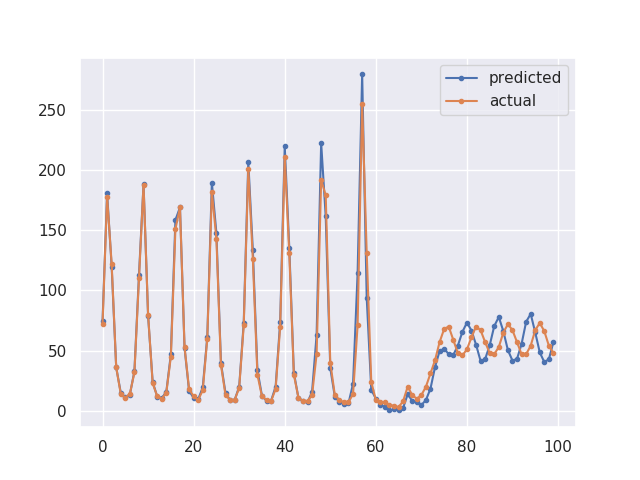
\includegraphics[width=\linewidth]{timeseries/LSTM_10_200_}          
        \end{subfigure}
        \begin{subfigure}{8cm}
            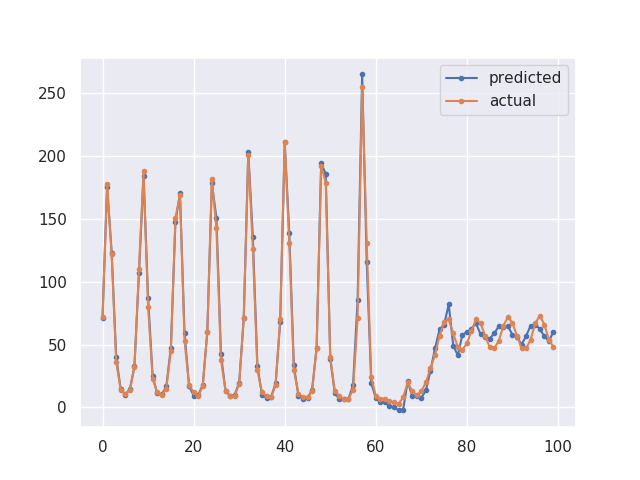
\includegraphics[width=\linewidth]{timeseries/LSTM_40_100_}            
        \end{subfigure}  

        \caption{Time series prediction with the MLP (a) and the LSTM (b) network }
                
        \label{fig:santafe1}
    \end{figure*}


       \begin{figure*}[]
        \begin{subfigure}{0.33\linewidth}
            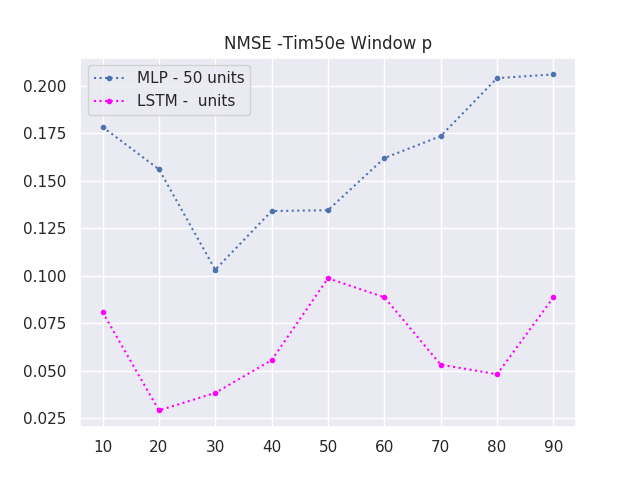
\includegraphics[width=\linewidth]{50}
            \caption{50 units}
        \end{subfigure}
        \begin{subfigure}{0.33\linewidth}
            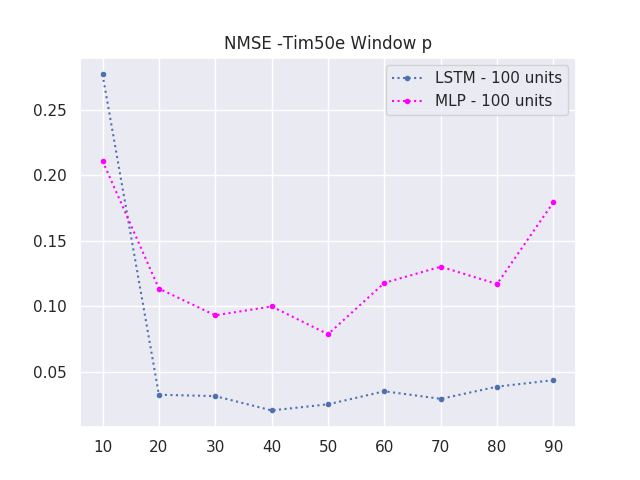
\includegraphics[width=\linewidth]{100}
            \caption{100 units}
        \end{subfigure}
        \begin{subfigure}{0.33\linewidth}
            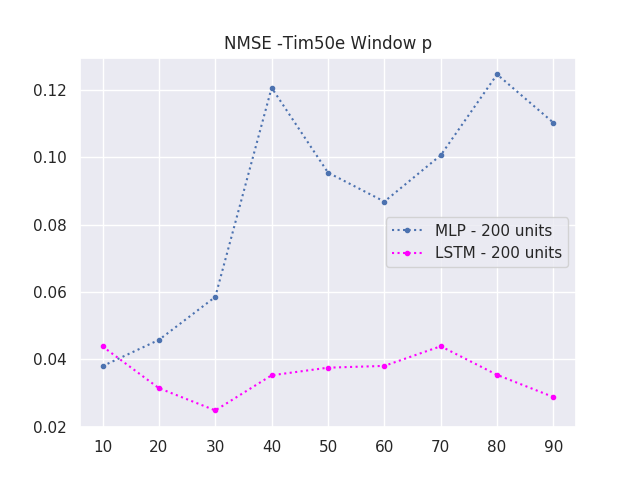
\includegraphics[width=\linewidth]{200}
            \caption{200 units}
        \end{subfigure}

\centering
	\begin{subfigure}{6cm}
            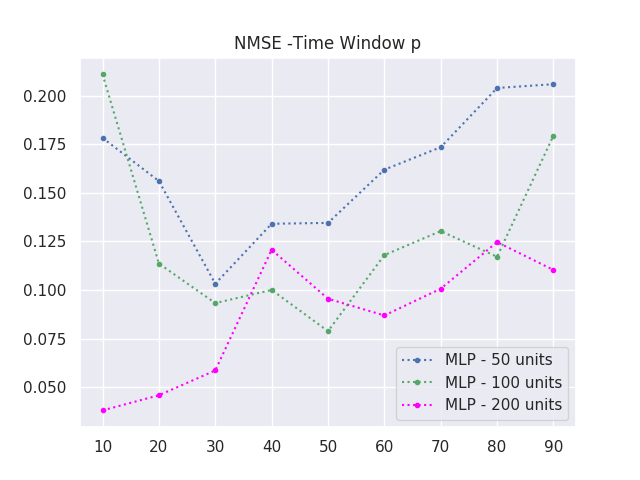
\includegraphics[width=\linewidth]{mlpsunits}          
        \end{subfigure}
        \begin{subfigure}{6cm}
            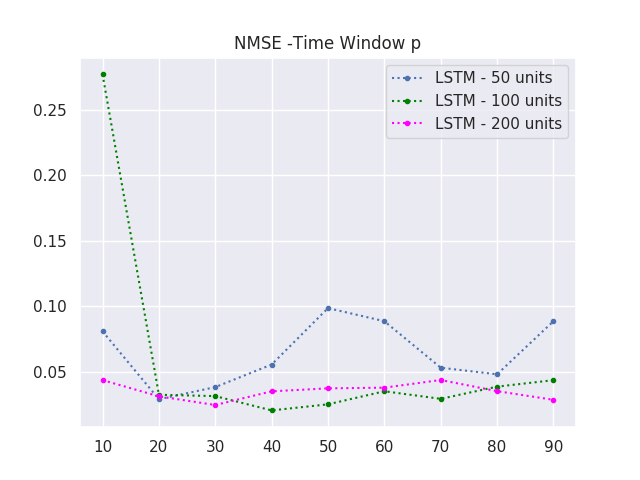
\includegraphics[width=\linewidth]{LSTMsunits}            
        \end{subfigure}  

        \caption{Normalized Mean Squared error (NMSE) against the selected time delay p for the MLP and LSTM with 50,100 and 200 hidden units  }
                
        \label{fig:rectune}
    \end{figure*}


%Figure~\ref{fig:tuning} shows the Mean Squared error loss in the validation set for epochs 0-500 measured while varying the number of neurons in the hidden layer. 
 
  
\subsubsection{Results and conclusions}


 While recurrent neural networks can perform better in some tasks than feedforward models by understanding sequential dependencies, their performance can be limited by the training algorithm used for optimization. A common problem is that of vanishing gradients that occurs when the values of the gradients computed during backpropagation get extremely small, thus allowing minor weight updates. 
One possible solution to this problem could to be use activation functions that have non-zero gradients over a large range of values. LSTM models tackle this problem from a different perspective. The gates of LSTM models control the flow of information to the hidden neurons and preserve the extracted features from previous states, making them more suitable to capture long term dependencies in the data.

A summary of the hyperparameters search results is shown in Figure~\ref{fig:rectune}. The Mean Root Squared Error is described as:

\begin{equation}
 RMSE = \frac{  \sum_{1}^{100}  \sqrt{ (\hat{y_k}-y_k )^2 }}{100}
\end{equation} The reported performance is the Normalized expression of equation 1 (NRMSE) which occurs by dividing the MSE by the average observation value. The NRMSE is averaged over 10 independent trials. The most important conclusion is that the LSTM architecture performs significantly better than the recurrent MLP for almost every combination of neurons and time delay $p$. The MLP reaches its best score of 0.037 when the time delay is $p=10$ and an architecture of 200 hidden neurons is used. This result indicates that using a large time delay in a simple recurrent model, may negatively impact the prediction ability of the network. This is not the case for the LSTM model, which achieves its best reported NRMSE score of 0.0207 by using an architecture of 100 hidden units and a time delay of 
$p =40$. A visualization of the prediction is shown in Figure~\ref{fig:santafe1}.


  



\section{Deep feature learning}
\subsection{Principal Component Analysis on Handwritten Digits}
Principal component analysis (PCA) is a dimensionality reduction technique that projects a set of $N$ data observations $\{x_i\}_{i=1}^N$ in a lower dimensional space while maximizing the variance of the projected data. The first step, usually involves standardization of the input vectors with a view to transform all the variables in the same range. In the next step, the the Covariance matrix $C=\{xx^T\}$ of the dataset is computed which contains all the possible covariance pairs of the initial variables. The covariance matrix expresses how the variables of the observations are varying from the mean with respect to each other and is symmetric with respect to the main diagonal. The eigenvectors of the Covariance matrix are the directions of maximal variance (e.g. more information) and are called principal components. Naturally, the eigenvalues represent the amount of variance that each principal component carries and can be used to rank the principal components in order of significance.

In this exercise, the objective is to perform PCA on handwritten images of the digit 3 taken from the US Postal Service database. The provided dataset includes 500 images of size $16 \times 16$ that have been reshaped to 256 dimensional vectors. Figure~\ref{fig:pca1} shows the  of the database (leftmost) and the visualizations of the first 4 principal components. After computing the eigenvectors and eigenvalues, a choice has to be made as to how many components are going to describe the encoded representation. Figure~\ref{fig:pca3} shows the cumulative explained variance ratio as a function of the number of components. This is computed by dividing the variance of each principal component to the total variance which is the sum of variances of all individual principal components. It is observed that the first 10 components contain 59\% of the variance, while we need around 100 components to describe close to 100\% of the variance. 

By selecting the first $k$ principal components the digit images are compressed and projected into a lower dimensional space. More specifically, this is done by multiplying the centered data matrix $X$  with a matrix $V$ containing the first $k$ eigenvectors. In order to reconstruct the images, we can simply use the feature matrix $V^T$ and multiply it with the projection, as 
$\hat{X}=XVV^T$. The final reconstruction matrix is obtained by adding the mean vector $\mu$ to the last expression. Figure~\ref{fig:pca3} shows the result of reconstructing a digit image by projecting it onto 4, 20, 80, and finally 256 principal components. By using more principal components, the reconstruction becomes better since we are imposing less sparsity constraints (e.g. the dimension of the compressed representation is closer to the original dimension).

The quality of the reconstruction error can be measured by computing the L2 norm $\frac{1}{N}\sum_{i=1}^{N}||x_i-\hat{x_i}||_2^2$. As expected, by using more principal components the reconstruction error becomes smaller. Figure~\ref{fig:pca3} shows the reconstruction error computed as a function of the number of principal components $k$. It is observed that as $k$ increases, the reconstruction error decreases since the components contain contain more variance and are able to better preserve the information contained in the encoded representation.



\begin{figure*}[!htb]
\centering
\minipage{0.07\textwidth}
  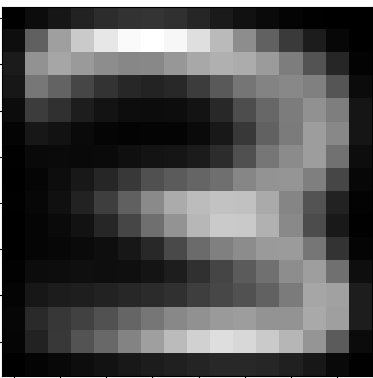
\includegraphics[width=\linewidth]{mean.png}
\endminipage
\vspace{1mm}
\minipage{0.07\textwidth}
  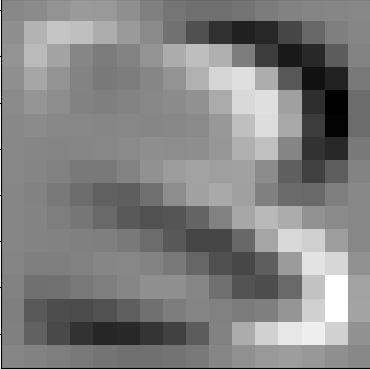
\includegraphics[width=\linewidth]{eigenvectors_0.png}
\endminipage
\vspace{1mm}
\minipage{0.07\textwidth}%
  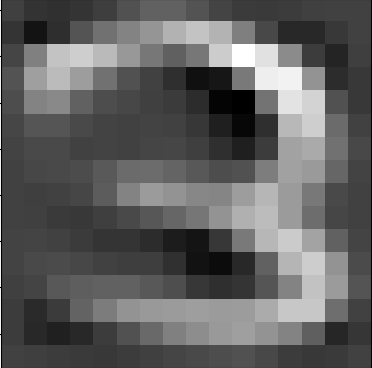
\includegraphics[width=\linewidth]{eigenvectors_1.png}
\endminipage
\vspace{1mm}
\minipage{0.07\textwidth}%
  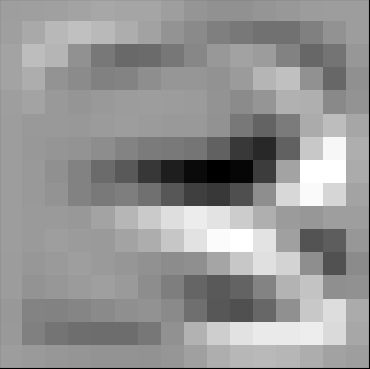
\includegraphics[width=\linewidth]{eigenvectors_2.png}
\endminipage
\vspace{1mm}
\minipage{0.07\textwidth}%
  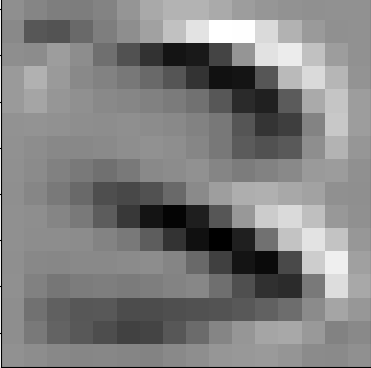
\includegraphics[width=\linewidth]{eigenvectors_3.png}
\endminipage

\centering
\minipage{0.07\textwidth}
  \includegraphics[width=\linewidth]{rec/4.png}
\endminipage
\vspace{1mm}
\minipage{0.07\textwidth}
  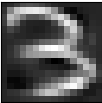
\includegraphics[width=\linewidth]{rec/20.png}
\endminipage
\vspace{1mm}
\minipage{0.07\textwidth}%
  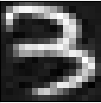
\includegraphics[width=\linewidth]{rec/80.png}
\endminipage
\vspace{1mm}
\minipage{0.07\textwidth}%
  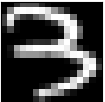
\includegraphics[width=\linewidth]{rec/256.png}
\endminipage
\caption{Top: mean image of the database and visualizations of the first 4 principal components (left to right). Bottom: Reconstructing the digit image by using 4, 20, 80 and 256 principal components (left to right)}
\label{fig:pca1}
\end{figure*}


 \begin{figure}
	\begin{subfigure}{8cm}
            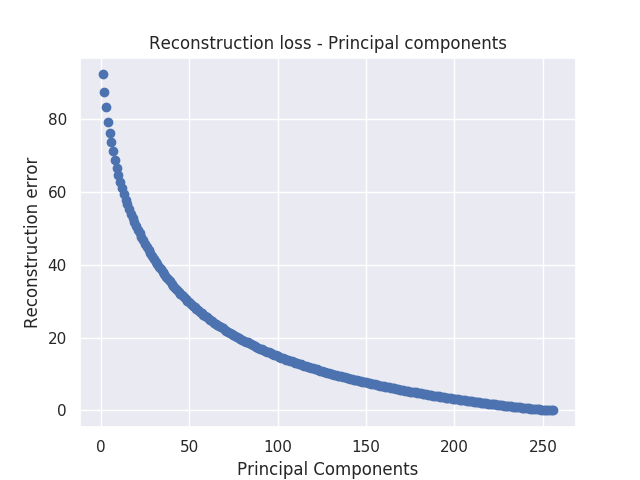
\includegraphics[width=\linewidth]{pcaloss}          
        \end{subfigure}
        \begin{subfigure}{8cm}
            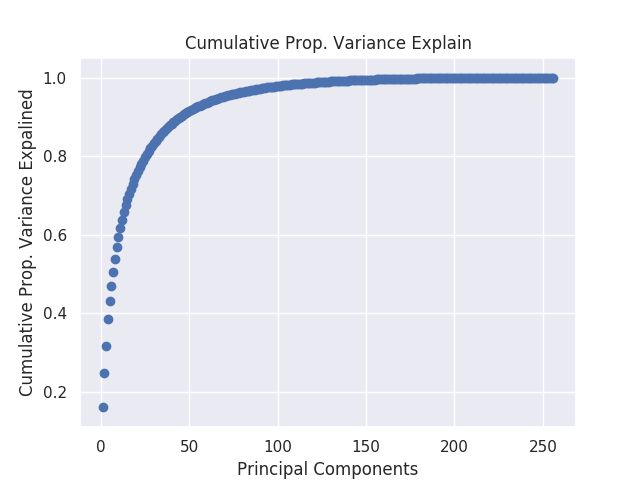
\includegraphics[width=\linewidth]{variance}            
        \end{subfigure}  
        \caption{Top: Reconstruction error, Bottom: Cumulative proportional variance explained}
                
        \label{fig:pca3}
    \end{figure}



\subsection{Stacked Autoencoders}


\subsubsection{Handwritten Digit Classification using Stacked Autoencoders}

\subsubsection{Stacked Autoencoders}
Similarly to PCA, autoencoders reduce the dimensionality of their input $x$ by constructing an internal compressed representation $z=G(x)$ in the hidden layer, which is typically smaller in size than the input layer. The network tries to generate a representation $\hat{x}=F(z)$ as close as possible to the original input and its trained in an unsupervised manner. In the case where the hidden layer is equal in size as the input layer, the network will simply learn the identity function and the learning problem becomes trivial. However, by imposing sparsity constraints, such as limiting the number of hidden units, the network can discover the underlying structure of the data and encode it in a lower dimensional representation.

A stacked autoencoder is a neural network consisting of multiple layers of sparse autoencoders in which the outputs of each layer is connected to the inputs of the successive layer. These models are typically trained in an unsupervised, greedy, layer-wise fashion. This is typically done by 
training the layer of each one of the stacked autoencoders separately and use it as input to the first layer of the next model. Moreover, the weights could potentially be used to initialize a deep neural network for a discriminative task (e.g. classification), since they have been optimized to encode the underlying patterns that describe the data. The output of the last autoencoder should be connected to a layer suitable for the task at hand, which in the case of image classification can be softmax layer. The softmax function simply takes as input a vector of $K$ real numbers, in this case the reshaped flattened images, and normalizes it into a probability distribution of $K$ probabilities. Finally, in most cases, the weights still need to be adjusted for the new task and the model is re-trained in a supervised manner.

\subsubsection{Experimental Setup \& Results}

In this exercise, the task is to train a stacked autoencoder to classify images representing handwritten digits. The methodolody followed to find the optimal values for different hyperparameters is similar to the one deployed in the exercises of the previous sections. Results are averaged over 10 runs during which the number of hidden units, the number of epochs and the number of layers are varied. The experiments involved training two different architectures, one with three and one with four hidden layers which are summarized in Table~\ref{tableaut}. In all cases, every successive layer is required to reduce the dimension of the input by a factor of 2. The first model, denoted as model A is comprised of two successive layers of 40 and 20 hidden units respectively and achieves an accuracy score of 0.9581. Raising the number of hidden units to 50 and 100 (model B) in the two successive layers yields a result of 0.9887. The final architecture, denoted as model C is comprised of 100 and 200 hidden units but does not produces an average better score than model B. Therefore model B is selected. 

Two MLP architectures comprised of one hidden layer with 100 units and two hidden layers with 100 hidden units were also trained for the task of digit classification. The network with one layer achieved an average score of 0.9712 while the architecture with 2 hidden layers achieved a score of 0.9789. This model is compared against model B and C since model A has a smaller number of parameters. The conclusion is that the MlP architectures performed worst than model B and C since the average accuracy result over 10 runs is notably smaller.

\begin{table}
\begin{subtable}[t]{0.48\textwidth}
\centering
%\begin{tabular}[t]{@{} l c *{3}{d{1.7}}d{3} @{}}
\begin{tabular}[t]{l l l l l l |l l}
\toprule
 \textbf{model A}  & units&    &accuracy\\
\midrule
  & 40 &  &0.9581 &\\
  & 20  & &\\
\midrule                                                  
   \textbf{model B} &units&&accuracy\\
\midrule
  & 50 &  & 0.9887 &\\
  &100  & &\\
  \midrule                                                  
   \textbf{model C} &units&&accuracy\\
\midrule
  & 100 &  & 0.9888&\\
  &200  & &\\  
\bottomrule
\end{tabular}
\end{subtable}
\caption{The deployed stacked autoencoder architectures. Classification accuracy is measured by averaging the results over 10 runs.}
\label{tableaut}
\end{table}

  





% Unsupervised training lets you show the network more data because it's much easier to get large unsupervised datasets than it is to get labeled ones.
%    You can use the pre-trained network as a "jumping off point" for training new classifiers so you don't have to start from scratch each time.
%

%So we first train the first
%autoencoder on the raw input to obtain the weights and biases from the input to the first hidden layer. Then we use this hidden
%layer as input to train the second autoencoder to obtain the weights and biases from the first to the second hidden layer. Repeat
%for subsequent layers, using the output of each layer as input for the subsequent layer. This method trains the parameters of each
%layer individually while freezing parameters for the remainder of the model. To produce better results, after this phase of training
%is complete, fine-tuning using backpropagation can be used to improve the results by tuning the parameters of all layers at the
%same time
%
%
%
% However, the weights still need to be adjusted for the new task and the sta
%
%cked l
% 
%
%
%
%The idea is that the weights learned in a unsupervised manner to minimize reconstruction error for the representation learning task offer a good starting point to initialize a network for a supervised discriminative task such as classification or similarity. I.e., the network learns something about the underlying distribution by looking at the unlabeled data, allowing it to discriminate between labeled data. However, the weights still need to be "fine-tuned" for this new task. So add a logistic regression layer on the top of the network and then do supervised learning with a labeled dataset. The fine tuning step will do gradient descent and adjust the weights for all layers in the network simultaneously.
%
%The advantages to this way of training neural nets are:
%
%    Unsupervised training lets you show the network more data because it's much easier to get large unsupervised datasets than it is to get labeled ones.
%    You can use the pre-trained network as a "jumping off point" for training new classifiers so you don't have to start from scratch each time.
%


\subsection{Convolutional Neural Networks}

\subsubsection{Convolutional Neural networks}
In this exercise, a pre-trained Convolutional Neural network (CNN) named AlexNet is deployed to classify three different classes ('airplane', 'ferry' and 'laptop'). The first two Convolutional layers are followed by Max Pooling layers, while the following three convolutional layers are connected directly. After the fifth convolutional layer, another Max Pooling layer is applied. The last three layers are fully connected layers, with the output being a softmax classifier with 1000 class labels. An important feature of this architecture is the use of 
 (Rectified Linear Unit) activation functions.

The input volume of ALexNet is 3-channel images of size $227 \times 227$. The parameters of the every convolutional layer are learnable filters that are connected through the full depth of the input volume. For example, every filter in the first convolutional layer has size of $11 \times 11  \times 3$ (i.e. the filters have 11 pixels width and height, and 3 since the input volume has 3 RGB color channels). Every filter in this layer can also be interpreted as a neuron that is connected to a local $11 \times 11$ area of the input volume and shares the shame $11 \times 11 \times 3$ weights with all neurons to the left and right spatially. The convolution operation computes dot products between the entries of the filter and the input at any position across the width and the height of the input volume. The output of one single filter is a two dimensional activation map that describes the reponse of this filter in every spatial location of the input volume. By introducing 96 such filters, the first convolutional layer introduces $11 \times 11 \times 3 \times 96$ weights and produces 96 two dimensional activation maps, one for each filter. Since each filter in the layer is convolved with a stride of 4, every produced two dimensional activation map will have a width and height of size $\frac{227-11}{4}+1 = 55$. Finally, stacking these 96 activation maps along the depth dimension produces an output volume of size $55 \times 55 \times 96$.

Between the first and the second convoultional layers there is one ReLU, one Max Pooling and one Batch normalization layer. The ReLU layer applies the function $f(x) = max(0,x)$ to the values of the input volume and represents the activation function of each of the 96 neurons of the first layer. The batch normalization layer, simply normalizes the output of the previous activation layer by subtracting the batch mean and dividing by the batch standard deviation.

 The Max pooling layer, operates independently along the depth dimension and further reduces the width and height of its input volume to  $\frac{55-3}{2}+1 = 27$ by reporting the maximum output within a rectangular neighborhood. The second convolutional layer uses a stride of 1 and does not further reduce the dimension of its input. The second max pooling layer that is applied afterwards reduces the input volume by $\frac{27-3}{2}+1 = 13$. The next 3 convolutional layers also use a stride of 1 and do not reduce the dimension of their input volume. The final Max pooling layer, reduces the dimension to $\frac{13-3}{2}+1 = 6$. The last three fully connected layers are comprised of 4096, 4096 and 1000 neurons respectively. Essentially, this means that the initial $227 \times 227 \times 3 = 154.587$ dimension of the input image is downsampled to a vector 154.587 times smaller with 1000 values. 
  
  
%\begin{figure*}
%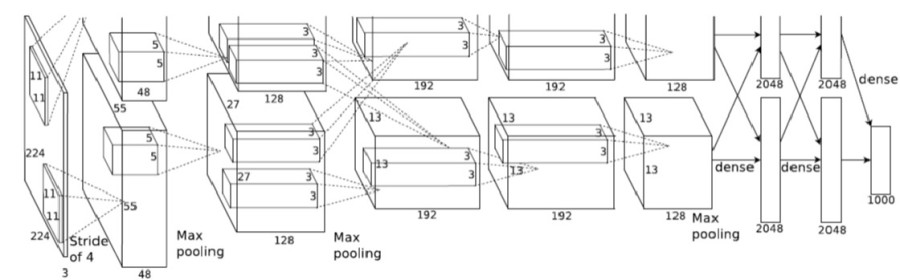
\includegraphics[width=\linewidth]{alexnet}
 %           \caption{The AlexNet architecture}
 %  \label{fig:alexnet}
 % \end{figure*}
  
\begin{figure*}
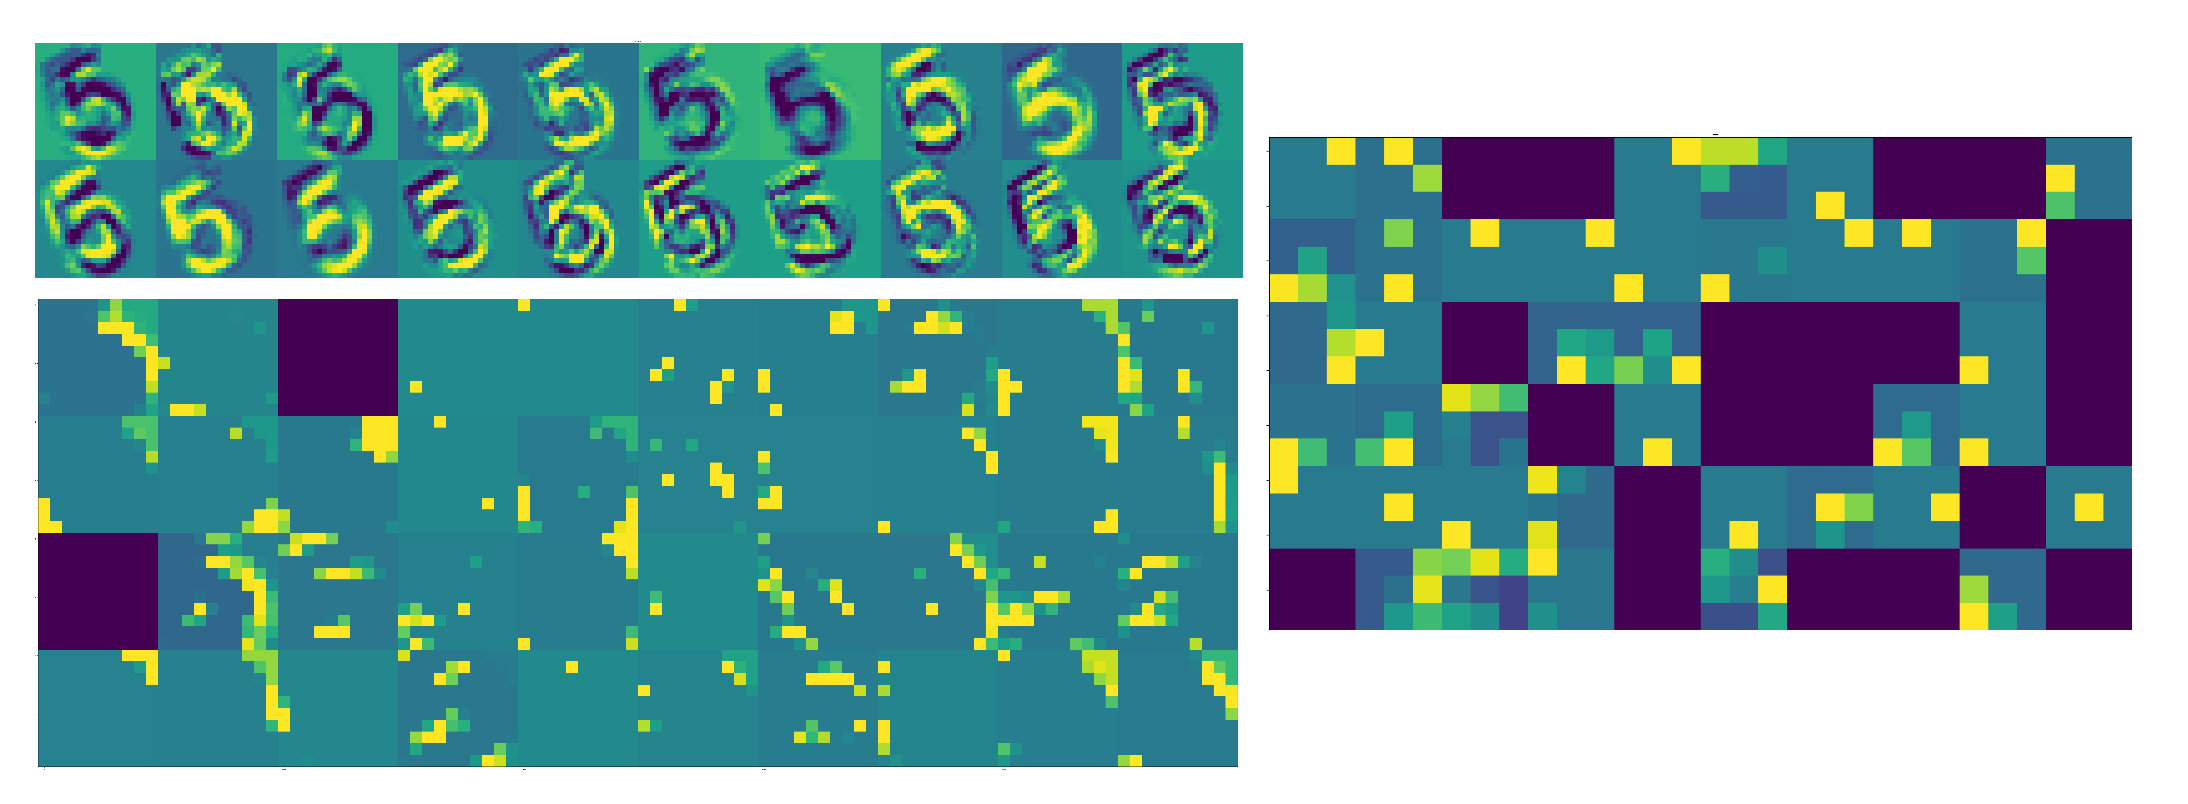
\includegraphics[width=\linewidth]{filters}
        \caption{Visualization of activation maps for the 20, 40 and 60 filters of yhe three convolutional layers of architecture E}
\label{fig:filters}
\end{figure*}
  
  
  
  
  
  
  
  
  
\subsubsection{Handwritten Digit Classification using Convoluational Neural Networks}
Deep Convolutional Neural Networks (CNNs) are widely used for image classification tasks. Despite their efficieny, finding the optimal architecture that works best for each problem still remains a challenging issue. The performance of CNNs can depend on several hyper-parameters such as the number of convolutional layers or the number of filters applied in each layer and their respective sizes. In this exercise, several experiments were made in order to find the most suitable CNN architecture that can accurately classify the USPS Digit dataset, which consists of 10.000 grayscale images, representing 10 handwritten digits - from 0 to 9. 

The data was randomly divided into training and test sets, so that each category in the training set has 750 images, and each category in the test set has 250 images. Three seperate set of experiments were conducted in which the the number of convolutional layers, the number of filters in each layer and the activation function applied after each convolution layer were varied. Results are presented in terms of classification accuracy by taking the maximum accuracy over 10 runs. Every training experiment was run for 60 epochs with a learning rate of $10^-3$. 

The deployed CNN architectures used in this task are summarized in Table~\ref{cnnt1}. The first three architectures, denoted by A, B and C, are comprised of one convolutional layer with 2, 5 and 20 filters repsectively, followed by a max pooling and a dense layer with softmax activation. Adding more filters to the convolutional layer will allow the network to learn different features and will thus increase the parameters and computation of the network as well as the depth of the output volume. Indeed, by increasing the number of parameters from 3K to 7K and finally 30K (for 2, 5 and 20 filters) classification accuracy is improved from 0.91 to 0.98 and finally 0.99.

A second set of experiments involved adding more convolution and pooling layers to the deployed architecure. The first layers of the CNN usually learn low level features (e.g. edges or curves) while upper layers learn to detect more complex high level features, possibly composed of low level representations. In table~\ref{cnnt3}, it is shown that adding more convolutional layers with gradually more filters, improves the classification accuracy from 0.9975 (2 convolutional layers), to 0.9995 (3 convolutional layers) to 1.0 (4 convolutional layers). 

Visualizing intermediate activations in a convolutional neural network involves displaying the features maps of a given input and examining how the input is decomposed into the different filters. A test image of the digit 5 was forwarded through the model D and the contents of each output layer are plotted as a 2D image. The first layer seems to be encoding the shape of the digit but as we go deeper in the convolutional layers, the activations become more abstract and less visuall interpretable as they describe more information reltaed to the class of the digit. Furthermore, it is shown that the sparsity of the activations increases as we go deeper in the network. In the first convolutional layer, every filter is activated by the input image but as we go deeper, more and more filters appear to be blank since the pattern encoded by these filters does not seem to be detected in the image. Some filter visualizations are shown in Figure~\ref{fig:filters}.

The final set of experiments involved exploring the behaviour of three different activation functions, namely ReLU, Leaky ReLU and PReLU for the architectures with 2 and 3 convolutional layers. The results are presented in Table~\ref{acti}. The function PReLU seems to have the best performance although the difference in accuracy is very small since the CNN are always able to achieve an excellent accuracy score.


\begin{table}
\begin{subtable}[t]{0.48\textwidth}
%\begin{tabular}[t]{@{} l c *{3}{d{1.7}}d{3} @{}}
\centering
\begin{tabular}[t]{l l l l l l |l l}
\toprule
 \textbf{model D} & activation &   params &accuracy\\
\midrule
  & ReLU &  18,770 & 0.9975 &\\
  &LeakyReLU & 18,770 & 0.9991& \\
    & PReLU  &   34,290  &  0.9995  \\
    
\midrule                                                  
   \textbf{model E} & activation &   params &accuracy\\
\midrule
  & ReLU &  31,030 & 0.9995 &\\
  &LeakyReLU & 31,030 & 1.0 & \\
    & PReLU & 88,190 &    1.0   &        \\
    
\bottomrule
\end{tabular}


\end{subtable}
\caption{Results for different activation functions}
\label{acti}
\end{table}

  











%%%%%%%%%%%%%%%%%%%%%%%%%%


\begin{table*}
\centering
%\begin{tabular}[t]{@{} l c *{3}{d{1.7}}d{3} @{}}
\begin{tabular}[t]{l l l l l l |l l}
\toprule
 \textbf{A} & layer &   kernel & filters & input & output & params &accuracy\\
\midrule
  & conv 1 &   5 x 5 &      2 &       28 x 28 x 2 & 24 x 24 x 2 &3,042& 0.9153\\
  & max pool &   2 x 2 &       &       24 x 24 x 2 & 12 x 12 x 2 \\
  &  dense &    &       &       288 & 10 \\

\midrule                                                  
  \textbf{B}    & conv 1 &   5 x 5 &      5 &       28 x 28 x 5 & 24 x 24 x 5 & 7,590 & 0.9878 \\
  & max pool &   2 x 2 &       &       24 x 24 x 5 & 12 x 12 x 5 \\
  &  dense &    &       &       720 & 10 \\

\midrule                                                  
   \textbf{C}    & conv 1 &   5 x 5 &      20 &       28 x 28 x 2 & 24 x 24 x 20 & 30,330 &0.9951 \\
  & max pool &   2 x 2 &       &       24 x 24 x 2 & 12 x 12 x 20 \\
  &  dense &    &       &       28880 & 20 \\

\bottomrule
\end{tabular}

\label{tab:table1_a}

\caption{Varying the number of filters with 1 convolutional layer}
\label{cnnt1}
\end{table*}





\begin{table*}
\centering

%\begin{tabular}[t]{@{} l c *{3}{d{1.7}}d{3} @{}}
\begin{tabular}[t]{l l l l l l |l l}
\toprule
 \textbf{D} & layer &   kernel & filters & input & output & params &accuracy\\
\midrule
  & conv 1 &   5 x 5 &      20 &       28 x 28 x 20 & 24 x 24 x 20 &18,770& 0.9975\\
  & max pool &   2 x 2 &       &       24 x 24 x 20 & 12 x 12 x 20 \\
    & conv 2 &   3 x 3 &    40   &       12 x 12 x 20 & 10 x 10 x 40 \\
      & max pool &   2 x 2 &       &       10 x 10 x 40 & 5 x 5 x 40 \\
  &  dense &    &       &       10010 & 10 \\

\midrule                                                  
  \textbf{E}     & conv 1 &   5 x 5 &      20 &       28 x 28 x 20 & 24 x 24 x 20 &31,030& 0.9995\\
  & max pool &   2 x 2 &       &       24 x 24 x 20 & 12 x 12 x 20 \\
    & conv 2 &   2 x 2 &    40   &       12 x 12 x 20 & 10 x 10 x 40 \\
      & max pool &   2 x 2 &       &       10 x 10 x 40 & 5 x 5 x 40 \\
       & conv 3 &   3 x 3 &    60   &       5 x 5 x 40 & 3 x 3 x 60 \\
  &  dense &    &       &       610 & 10 \\

\midrule                                                  
    \textbf{F}  & conv 1 &   5 x 5 &      20 &       28 x 28 x 20 & 24 x 24 x 20 &74,510&  1.0\\
  & max pool &   2 x 2 &       &       24 x 24 x 20 & 12 x 12 x 20 \\
    & conv 2 &   2 x 2 &    40   &       12 x 12 x 20 & 10 x 10 x 40 \\
       & conv 3 &   3 x 3 &    60   &       5 x 5 x 40 & 3 x 3 x 60 \\
       & conv 3 &   3 x 3 &    60   &       3 x 3 x 60 & 1 x 1 x 80 \\
  &  dense &    &       &       810 & 10 \\
\bottomrule
\end{tabular}



\caption{Varying the number of convolutional layers}
\label{cnnt3}
\end{table*}






\section{Generative models}

\subsection{Restriced Boltzmann Machines}

A restricted Boltzmann Machine (RBM) is a stochastic, recurrent fully connected neural network.  The difference with a Hopfield network that was studied in section 2.1 is the use of stochastic units that output the probability of being in a particular state.
 The connection between two neurons is symmetric such that $w_{ij}=w_{ji}$, where $w_{ij}$ is the connection between neuron $i$ and $j$. The model defines a probability distribution over the different possible states. The probability of a state $v$ is:
\begin{equation}
P(v,h;\theta)=\frac{1}{Z(\theta)}exp(E(v,h;\theta)
\end{equation}
where $E(v,h;\theta)$ is the energy function of the model defined as $E(v,h;\theta)=-v^TWh-b^Tv-a^Th$. In the previous equations $\theta$ denotes the parameters of the model consisting of the weight matrix $W$, the bias $b$ and the offset $a$. The RBM model provides a representation of the learned distribution. By iteratively adjusting the weights, an RBM learns to approximate the original distribution of the data and the activations of the hidden layer encode the structure of the input.

The reconstruction task is different from the discriminative task performed by classification which maps inputs to labels or from regression which predicts outputs of real values. Therefore, it is a generative model that samples from the learned distribution. The term "restricted" describes the absence of connections between the layer of hidden units $h$ and visible units $v$ which eventually makes the hidden variables $h$ independent given the state of the visible variables $v$. The independence of variables allows to sample the states of all variables jointly instead of sampling new values from every variable every time.
The unknown parameters can be learned by performing a log likelihood
estimation using the following update rule: 
\begin{equation}
\Delta W=\alpha (E_{Pdata}[vh^T]-E_{PT}[vh^T])
\end{equation}
where $P_T$ denotes a distribution defined by Gibbs sampling. The model is trained in an unsupervised manner in a sense that the hidden representations are constructed from unlabeled data. 

In this exercise, an RBM model is trained to reconstruct digits from the MNIST database \cite{mnist}. The objective is to behave the network's behavior by varying the values of the hyperparameters that are described below.
\\
\textbf{Number of hidden neurons}
From a machine learning point of view an image is a point in the $N$ dimensional space where $N$ is equal to the number of pixel values. In this case the network consists of $28 \times 28 = 784 $ visible neurons. The number of hidden neurons is a hyperparameter that can be controlled and is related to the number of features that the network is going to extract. A small number of neurons leads to underfitting since the model does not have a lot of flexibility and is not able to approximate the distribution of the input data. This situation is depicted in Figure~\ref{fig:rbm}. The reconstructions do not correspond to digits but instead to abstract shapes. On the other hand, a very large number of parameters leads to overfitting since the model memorizes the input digits. An example of overfitting is illustrated in Figure~\ref{fig:rbm2}. The reconstructions correspond to digits but seem very similar since the network has memorized the training input.
\\
\textbf{Learning Rate} The learning rate is simply the parameter $a$ in equation 5. A very small value will allow minor weight updates which will make the optimization process very slow. On the other hand, a very large value will allow major weight updates which may result in the algorithm not converging to the optimum of the objective function.
Increasing the learning rate to values more than 0.4 or lowering it below 0.05 makes the training very unstable.

\begin{figure}[!htb]
\centering
\minipage{0.07\textwidth}
  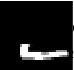
\includegraphics[width=\linewidth]{un1.jpg}
\endminipage
\vspace{1mm}
\minipage{0.07\textwidth}
  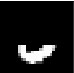
\includegraphics[width=\linewidth]{un2.jpg}
\endminipage
\vspace{1mm}
\minipage{0.07\textwidth}%
  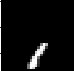
\includegraphics[width=\linewidth]{un3.jpg}
\endminipage

\caption{Examples of underfitting when using a very small number of hidden units}
\label{fig:rbm}
\end{figure}



\begin{figure}[!htb]
\centering
\minipage{8cm}
  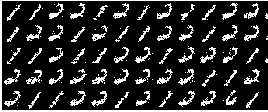
\includegraphics[width=\linewidth]{over.png}
\endminipage

\caption{Examples of overfitting when using a very large number of hidden units}
\label{fig:rbm2}
\end{figure}


%If the learning rate is much too large, the reconstruction error usually increases dramatically and the
%weights may explode.
%If the learning rate is reduced while the network is learning normally, the reconstruction error
%will usually fall significiantly. This is not necessarily a good thing. It is due, in part, to the smaller
%noise level in the stochastic weight updates and it is generally accompanied by slower learning in
%the long term. Towards the end of learning, however, it typically pays to decrease the learning rate.
%Averaging the weights across several updates is an alternative way to remove some of the noise from
%the final weights.




\textbf{Iterations} The number of iterations refers to the iterations the algorithm is making over the training data during training. Similarly as the parameter "number of epochs" that was discussed in section 1.1.1, the number of iterations should be large enough so that the algorithm can converge to the optimum.


\section{Deep Boltzmann Machines}
A deep Boltzman machine (DBM) consisting of $n$ hidden layers is a RBM model that uses multiple layers of hidden units so that the following probability is assigned to each visible state $v$:

\begin{equation}
P(v;\theta)=\frac{1}{Z(\theta)} \sum_{h^1,...,h^n}{exp(-E(v,h^1,...,h^n;\theta))}
\end{equation}
where the variables $h^1,...h^n$ refer to the hidden feature representations the network is expected to learn. Similarly to other deep learning models like deep CNNs or deep belief networks, DBMs can learn internal representations that are increasingly complex, with low level layers encoding simple features (e.g. edges) and deeper layers encoding high level abstractions. Consequently, in this case the first layer of hidden features is expected to capture the correlations between the visible units. Deeper layers are expected to capture high-order correlations between the hidden features in the layer below.
Figure~\ref{fig:dpm} shows a visualization of the weights learned in the first and the second layer of a DPM. 

    \begin{figure*}[]
        \centering
        \begin{subfigure}{0.30\linewidth}
            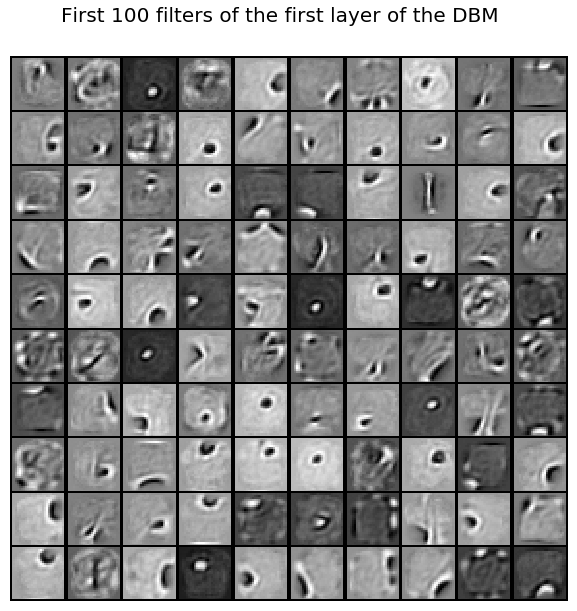
\includegraphics[width=\linewidth]{dpm/shallow}
            \caption{1st layer}
        \end{subfigure}
         \begin{subfigure}{0.30\linewidth}
            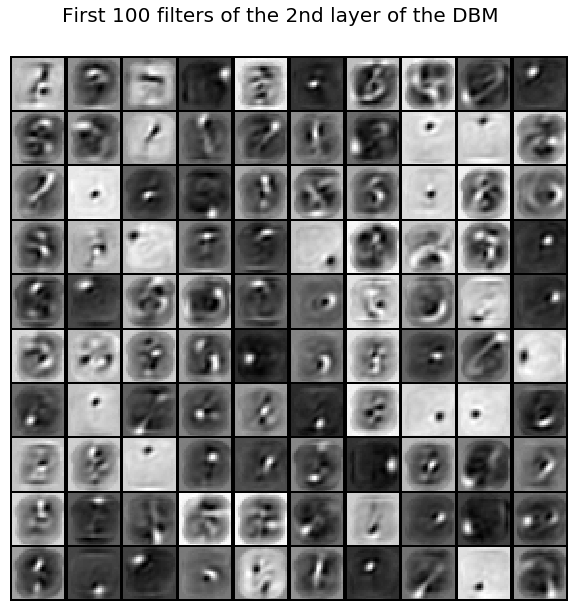
\includegraphics[width=\linewidth]{dpm/deep}
            \caption{2nd layer}
        \end{subfigure}  
        		        
        \caption{Visualizing the filters learned in the first layer (a) and in the second layer (b) of a Deep Restricted Boltzman Machine}
        \label{fig:dpm}
\end{figure*}

\section{Generative Adversarial Networks}

\subsection{Deep convolutional generative adversarial network (DCGAN)}




In this exercise, the objective is to train a Deep convolutional generative adversarial network (DCGAN) in the Cifar-10 dataset \cite{cifar}. The discriminator samples noise $z$ and tries to generate an image $x=G(z;\theta)$ where $\theta$ refers to the parameters of the model. The generator attempts to distinguish between samples drawn from the training data and samples drawn from the generator and gives a probability $D(x;\theta^{(D)}$ that indicates whether the image $x$ is a real training example or a fake example generated by the generator.  A DCGAN model will therefore transofrm the distribution of the training samples into a different distribution by applying augmentation to each source of variance that describes the data. 

The discriminator and generator compete against the other in a zero sum game where every network is trying to maximize its own payoff. This means that improvement in one network will cause the other network to deteriorate. Both the discriminator and the generator should however converge to some permanent parameters and one should regularly check the generated samples to evaluate the quality of the learning process. Figure~\ref{accs} shows the accuracy of the discriminator and the generator in a training of 80K iterations. Finally, in the context of GANs, overfitting can arise if the  generators mimics the training data exactly and ignores any attempts at adding stochastic changes to the training images. 


A classical problem that occurs in GANs is that of mode collapse that 
occurs when the generator generates a limited diversity of samples regardless of the input. The effect of this is that the discriminator will only discriminate between a small set of examples and both networks fall into a loop and will not converge. In this case, this phenomenon was not observed and the learning process was balanced.

\textbf{The generator}
The deployed generator architecture is composed of one fully connected and 3 convolutional layers. The first layer which is the fully connected layer takes as input a uniform noise distribution which is a 16384 dimensional vector. The representation is then reshaped to a $256 \times 8 \times 8$ volume and forward passed to 4 successive convolutional layers. In the provided code the three convolutional layers were applying 128, 64 and 32 filters respectively. The number of filters was doubled so as to have 256 filters in the first, 128 in the second and 64 filters in the third convolutional layer. The first two convolutional layers have a ReLU activation function while the last activation is the tanh function. The final layer of the network outputs a representation of size $32 \times 32 \times 3$, where the three dimensional depth corresponds to the three RBG channels of the image. 

\textbf{The discriminator} The discriminator is implemented as a deep CNN with 4 convolutional layers and one fully connected layer. Since the discriminator will attempt to distinguish between samples drawn from the training data and samples drawn from the generator the input size should be the same as the output size of the generator, that is $32 \times 32 \times 3$. The network is composed of 4 convolutional layers interspersed by dropout layers and a final fully connected layer. Since there is no use of max pooling layers, the dropout layers are used to prevent overfitting. The dropout layers probabilistically remove some of the interconnection weights and reduce the number of input activations that the next layer accepts. Moreover, after every convolutional layer there is a batch normalization layer that normalizes the output of a previous activation layer by subtracting the batch mean and by dividing by the batch standard deviation. The activation function of each convolutional layer is the Leaky ReLU activation function. Since the last layer should output a value that corresponds to probability, the sigmoid activation function is used that shifts the outputs in the range of $[0,1]$. The number of learnable filters in each convolutional layer was changed to 64, 128, 256 and 512.

    \begin{figure}[]
        \centering
     \begin{subfigure}{8cm}
          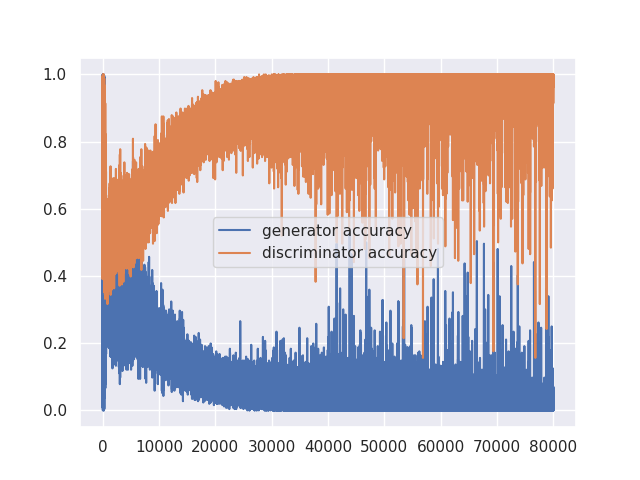
\includegraphics[width=\linewidth]{accs}
     \end{subfigure}

  	        
        \caption{Training a GAN in cifar-10}
        \label{accs}
\end{figure}

Both networks were trained using Adam optimizer with a learning rate of 0.0002. The parameter batch size refers to the number of samples that will be propagated through the network before every weight update takes place. For example if we set the batch size to 32 the algorithm will take the first 32 samples from th training dataset and will train the network. Next, the second 32 samples will be used for training. A common practice is to set the number of iterations equal to the number of training samples divided by the batch size so as to use all of the available training samples. Using large mini-batches usually scale up image classification tasks and improve the speed of training. \cite{large}. Since the discriminator behaves as an image classifier, a large batch size should have a positive impact. However, the training of GANs is a slightly different process than the training of a CNN classifier since the learning can diverge and for this reason  this question still remains open.
The batch size of this experiment was set to 128. Figure~\ref{fig:gan} shows the generated images during different number of iterations. 


    \begin{figure*}[]
        \centering
     \begin{subfigure}{16cm}
          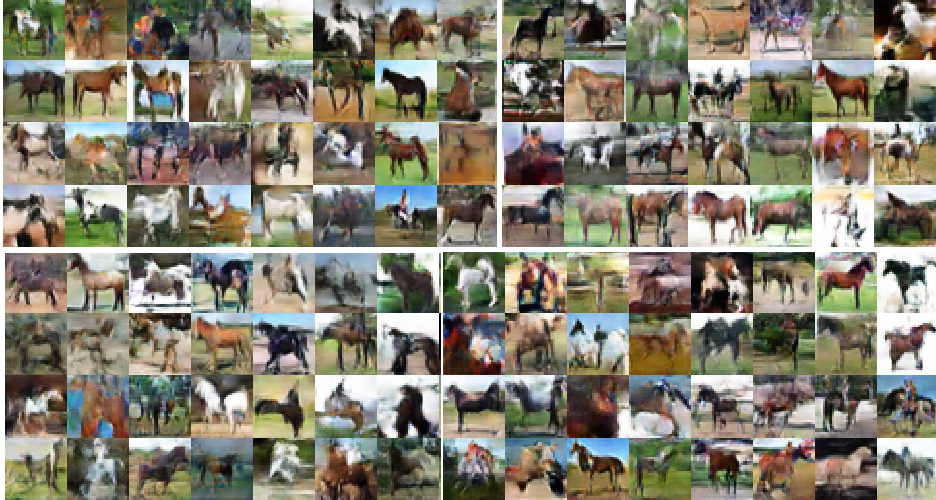
\includegraphics[width=\linewidth]{horse}
     \end{subfigure}

     
		        
        \caption{Synthetically generated images of horses}
        \label{fig:gan}
\end{figure*}



\subsection{Optimal Transport}
This exercise is concerned with the problem of color transfer. The goal of color transfer is to impose the look of one image to another by transferring the color palette of the first image to the second.
In other words the color distribution of the new image has to be as close as possible to the source image. The estimation of the optimal transport plan can be used to solve the problem of color transfer. The Wasswerstein distance is a metric for comparing distributions that may not have the same statistical properties and can be computed by minimizing the transport cost. These distances measure the amount of "work" that is needed to move all the mass that is contained in one distribution into the other.

In this exercise, we experiment with two different optimal transport algorithms one that uses the Wasserstein metric and one that uses the 
Sinkhorn distance. The results of the two algorithms are shown in Figure~\ref{fig:op}. The Sinkhorn metric performs better since the transfer is more smooth. This can attributed to the fact that the distance between the two distributions is regularized by the entropy term. The entropy term is often used to measure the level of uncertainty or unpredictability of a probability distribution. In contrast to the Wasserstein distance, the Sinkhorn distance is more smooth and more suitable for minimization problems. The optimal transport computation become a differentiable and unconstrained convex optimization problem which is solved iteratively using the Sinkhorn algorithm.

    \begin{figure*}[]
        \centering
        \begin{subfigure}{0.50\linewidth}
            \includegraphics[width=\linewidth]{op}
   
        \end{subfigure}	        
        \caption{Color transfer with Wasserstein and Sinkhorn algorithms}
        \label{fig:op}
\end{figure*}

\subsection{Comparison of a fully connected minimax GAN and Wasserstein GAN}
In this exercise, a fully connected minimax GAN and a Wasserstein GAN network (WGAN) are trained on the MNIST database. As previously mentioned the Wasserstein distance is a method to estimate the dissimilarity between two multidimensional distributions of data. The Wasserstein GAN redesigns the loss function and tries to minimize an approximation of this distance. The main advantage of WGAN network is that it does not assume that there is a balance in the training of the discriminator and the generator. The cost function that is being optimized has a smoother gradient which is always a desired property of every gradient based optimization scheme. This results in the WGAN network learning independently of the performance of the generator. 

 A minmax GAN model may also suffer from the problem of weight clipping that happens when all the weights are trapped in a specific range of $[min,max]$ values. As a result, the GAN is not able to model complex relations among the data since the structure it is trying to capture gets too restricted. Another symptom of weight clipping is that it may lead to vanishing or exploding gradients which makes the learning process impossible. The problem of weight clipping is solved by introducing a weight penalty mechanism that restricts some gradients to have a norm of 1. Another great advantage of WGANs over minmax GANs is that the training is much more stable and as a result less hyperparameter tuning is required. This means that the architecture of the network is not as important as it is in minmax GANs and high quality results can be achieved more easily. The reconstruction results are illustrated in Figure~\ref{fig:last}. Clearly the reconstruction produced by the WGAN is less noisy and more clear.






        \begin{figure*}[]
        \centering
    
         \begin{subfigure}{0.40\linewidth}
            \includegraphics[width=\linewidth]{gans/minmax}
            \caption{WGAN}
        \end{subfigure}  
        \begin{subfigure}{0.40\linewidth}
            \includegraphics[width=\linewidth]{gans/wgan}
            \caption{minmax GAN}
        \end{subfigure}
		        
        \caption{Comparing the performance of WGAN and minmax GAN}
        \label{fig:last}
\end{figure*}
%fully connected as it is just a matrix multiplication, but the result is reshaped into a 4-dimensional
%tensor and used as the start of the convolution stack. For the discriminator, the last convolution layer
%is flattened and then fed into a single sigmoid output. See Fig. 1 for a visualization of an example
%model architecture



%Why are hidden layers useful? The reason is that if we have no hidden layers and map directly from inputs to output, each input’s contribution on the output is independent of the other inputs. In real-world problems, input variables tend to be highly interdependent and they affect the output in combinatorially intricate ways. The hidden layer neurons allow us to capture subtle interactions among our inputs which affect the final output downstream. Another way to interpret this is that the hidden layers represent higher-level “features” or attributes of our data. Each of the neurons in the hidden layer weigh the inputs differently, learning some different intermediary characteristic of the data, and our output neuron is then a function of these instead of the raw inputs. By including more than one hidden layer, we give the network an opportunity to learn multiple levels of abstraction of the original input data before arriving at a final output. This notion of high-level features will become more concrete in the next chapter when we look closely at the hidden layers.
%
%Recall also that activation functions expand our capacity to capture non-linear relationships between inputs and outputs. By chaining multiple non-linear transformations together through layers, this dramatically increases the flexibility and expressiveness of neural networks. The proof of this is complex and beyond the scope of this book, but it can even be shown that any 2-layer neural network with a non-linear activation function (including sigmoid or ReLU) and enough hidden units is a universal function approximator, that is it’s theoretically capable of expressing any arbitrary input-to-output mapping. This property is what makes neural networks so powerful.
%
%





\bibliographystyle{IEEEtran}  
\bibliography{fdr_bib} 


\newpage
\clearpage
\appendix
 
\onecolumn

\newpage







  
     \begin{figure*}[]
 

        \begin{subfigure}{0.33\linewidth}
            \includegraphics[width=\linewidth]{Regression_3_layers50}
           
        \end{subfigure}
        \begin{subfigure}{0.33\linewidth}
            \includegraphics[width=\linewidth]{Regression_3_layers100}
            
        \end{subfigure}
		  \begin{subfigure}{0.33\linewidth}
            \includegraphics[width=\linewidth]{Regression_3_layers200}
           
        \end{subfigure}


        \begin{subfigure}{0.33\linewidth}
            \includegraphics[width=\linewidth]{3_layers50}
            \caption{50}
        \end{subfigure}
        \begin{subfigure}{0.33\linewidth}
            \includegraphics[width=\linewidth]{3_layers100}
            \caption{100}
        \end{subfigure}
		  \begin{subfigure}{0.33\linewidth}
            \includegraphics[width=\linewidth]{3_layers200}
            \caption{200}
            
        \end{subfigure}
        
	
        \caption{Predicted values against actual values for the MLP with 3 hidden layers (first row). Mean squared error against number of epochs (second row). The number of hidden neurons in each layer are varied from 25 (a) to 200 (b) and 200 (c).}        
                
        \label{fig:reg2}
    \end{figure*}     

\begin{figure*}
\centering
	\begin{subfigure}{6cm}
            \includegraphics[width=\linewidth]{optimizers_train}          
        \end{subfigure}
        \begin{subfigure}{6cm}
            \includegraphics[width=\linewidth]{optimizers_tval}            
        \end{subfigure}  

        \caption{Training, validation and test surfaces consisting of 1000 data points each (first row). Training and validation performance for Adam, Adadelta, Adagrad, Nadam and Adamax (second row). }
                
        \label{fig:surface}
    \end{figure*}

   \centering
\begin{table}
\centering
\begin{subtable}[t]{0.48\textwidth}
%\begin{tabular}[t]{@{} l c *{3}{d{1.7}}d{3} @{}}
\centering
\begin{tabular}[t]{l l l l l l l l l}
\toprule

\# units & params &$MAE$ &   $MSE$  &$R^2$\\
\midrule

                                          
 50  &2.751 &0.070 &0.0109  &0.5998 \\
                                               
 100 & 10.501 &0.0313 &   0.0022&0.9181 \\
 200 &41.001 &0.0196&  0.0008 &0.9676 \\
 \\



\bottomrule
\end{tabular}
\end{subtable}
\caption{Performance of regression measured by reporting the mean values for the Mean absolute error (MAE), Mean squared error (MSE), and $R^2$ over 10 runs. The deployed architecture consists of 3 hidden layers that have an equal amount of neurons in each layer.\\
 }
\label{fig:reg}
\end{table}








\end{document}


